%\pdfoutput=1
% Uncomment line above if submitting to arXiv and using pdflatex

% $Id: main.tex 33016 2013-03-25 11:27:03Z mamartin $
% ============================================================================
% Purpose: Template for LHCb documents
% Authors: Tomasz Skwarnicki, Roger Forty, Ulrik Egede
% Created on: 2010-09-24
% ============================================================================
\documentclass[12pt,a4paper]{article}
% For two column text, add "twocolumn" as an option to the document
% class. Also uncomment the two "onecolumn" and "twocolumn" lines
% around the title page below.

% Variables that controls behaviour
\usepackage{ifthen} % for conditional statements
\newboolean{pdflatex}
\setboolean{pdflatex}{true} % False for eps figures 
\usepackage{booktabs} % useful for tabs
\usepackage{multirow} % useful for tabs
\usepackage{rotating}	
\newboolean{articletitles}
\setboolean{articletitles}{true} % False removes titles in references

\newboolean{uprightparticles}
\setboolean{uprightparticles}{false} %True for upright particle symbols

% THis file contains all the default packages and modifications for
% LHCb formatting

%% %%%%%%%%%%%%%%%%%%
%%  Page formatting
%% %%%%%%%%%%%%%%%%%%
\textheight=230mm
\textwidth=160mm
\oddsidemargin=7mm
\evensidemargin=-10mm
\topmargin=-10mm
\headsep=20mm
\columnsep=5mm
\addtolength{\belowcaptionskip}{0.5em}

\renewcommand{\textfraction}{0.01}
\renewcommand{\floatpagefraction}{0.99}
\renewcommand{\topfraction}{0.9}
\renewcommand{\bottomfraction}{0.9}


\setlength{\hoffset}{-2cm}
\setlength{\voffset}{-2cm}
% Page defaults ...
\topmargin=0.5cm
\oddsidemargin=2.5cm
\textwidth=16cm
\textheight=22cm
% Allow the page size to vary a bit ...
\raggedbottom
% To avoid Latex to be too fussy with line breaking ...
\sloppy

%% %%%%%%%%%%%%%%%%%%%%%%%
%% Packages to be used
%% %%%%%%%%%%%%%%%%%%%%%%% 
\usepackage{microtype}
\usepackage{lineno}  % for line numbering during review
\usepackage{xspace} % To avoid problems with missing or double spaces after
                    % predefined symbold


%% Graphics
\usepackage{graphicx}  % to include figures (can also use other packages)
\usepackage{color}
\usepackage{colortbl}
\graphicspath{{./figs/}} % Make Latex search fig subdir for figures

%% Math
\usepackage{amsmath} % Adds a large collection of math symbols
\usepackage{amssymb}
\usepackage{amsfonts}
\usepackage{upgreek} % Adds in support for greek letters in roman typeset

%% fix to allow peaceful coexistence of line numbering and
%% mathematical objects
%% http://www.latex-community.org/forum/viewtopic.php?f=5&t=163
%%
\newcommand*\patchAmsMathEnvironmentForLineno[1]{%
\expandafter\let\csname old#1\expandafter\endcsname\csname #1\endcsname
\expandafter\let\csname oldend#1\expandafter\endcsname\csname
end#1\endcsname
 \renewenvironment{#1}%
   {\linenomath\csname old#1\endcsname}%
   {\csname oldend#1\endcsname\endlinenomath}%
}
\newcommand*\patchBothAmsMathEnvironmentsForLineno[1]{%
  \patchAmsMathEnvironmentForLineno{#1}%
  \patchAmsMathEnvironmentForLineno{#1*}%
}
\AtBeginDocument{%
\patchBothAmsMathEnvironmentsForLineno{equation}%
\patchBothAmsMathEnvironmentsForLineno{align}%
\patchBothAmsMathEnvironmentsForLineno{flalign}%
\patchBothAmsMathEnvironmentsForLineno{alignat}%
\patchBothAmsMathEnvironmentsForLineno{gather}%
\patchBothAmsMathEnvironmentsForLineno{multline}%
}

% Get hyperlinks to captions and in references.
% These do not work with revtex. Use "hypertext" as class option instead.
\usepackage{hyperref}    % Hyperlinks in references
\usepackage[all]{hypcap} % Internal hyperlinks to floats.

%%% $Id: lhcb-symbols-def.tex 30551 2013-01-25 19:09:21Z uegede $
%%% ======================================================================
%%% Purpose: Standard LHCb aliases
%%% Author: Originally Ulrik Egede, adapted by Tomasz Skwarnicki for templates,
%%% rewritten by Chris Parkes
%%% Maintainer : Ulrik Egede (2010 - 2012)
%%% =======================================================================

%%% To use this file outside the normal LHCb document environment, the
%%% following should be added in a preamble (before \begin{document}
%%%
%%%\usepackage{ifthen} 
%%%\newboolean{uprightparticles}
%%%\setboolean{uprightparticles}{false} %Set true for upright particle symbols
%%% \usepackage{xspace} 
%%% \usepackage{upgreek}

%%%%%%%%%%%%%%%%%%%%%%%%%%%%%%%%%%%%%%%%%%%%%%%%%%%%%%%%%%%%
%%%
%%% The following is to ensure that the template automatically can process
%%% this file.
%%%
%%% Add comments with at least three %%% preceding.
%%% Add new sections with one % preceding
%%% Add new subsections with two %% preceding
%%%%%%%%%%%%%%%%%%%%%%%%%%%%%%%%%%%%%%%%%%%%%%%%%%%%%%%%%%%%

%%%%%%%%%%%%%
% Experiments
%%%%%%%%%%%%%
\def\lhcb {\mbox{LHCb}\xspace}
\def\ux85 {\mbox{UX85}\xspace}
\def\cern {\mbox{CERN}\xspace}
\def\lhc    {\mbox{LHC}\xspace}
\def\atlas  {\mbox{ATLAS}\xspace}
\def\cms    {\mbox{CMS}\xspace}
\def\babar  {\mbox{BaBar}\xspace}
\def\belle  {\mbox{Belle}\xspace}
\def\aleph  {\mbox{ALEPH}\xspace}
\def\delphi {\mbox{DELPHI}\xspace}
\def\opal   {\mbox{OPAL}\xspace}
\def\lthree {\mbox{L3}\xspace}
\def\lep    {\mbox{LEP}\xspace}
\def\cdf    {\mbox{CDF}\xspace}
\def\dzero  {\mbox{D0}\xspace}
\def\sld    {\mbox{SLD}\xspace}
\def\cleo   {\mbox{CLEO}\xspace}
\def\argus  {\mbox{ARGUS}\xspace}
\def\uaone  {\mbox{UA1}\xspace}
\def\uatwo  {\mbox{UA2}\xspace}
\def\tevatron {Tevatron\xspace}

%% LHCb sub-detectors and sub-systems

\def\pu     {PU\xspace}
\def\velo   {VELO\xspace}
\def\rich   {RICH\xspace}
\def\richone {RICH1\xspace}
\def\richtwo {RICH2\xspace}
\def\ttracker {TT\xspace}
\def\intr   {IT\xspace}
\def\st     {ST\xspace}
\def\ot     {OT\xspace}
\def\Tone   {T1\xspace}
\def\Ttwo   {T2\xspace}
\def\Tthree {T3\xspace}
\def\Mone   {M1\xspace}
\def\Mtwo   {M2\xspace}
\def\Mthree {M3\xspace}
\def\Mfour  {M4\xspace}
\def\Mfive  {M5\xspace}
\def\ecal   {ECAL\xspace}
\def\spd    {SPD\xspace}
\def\presh  {PS\xspace}
\def\hcal   {HCAL\xspace}
\def\bcm    {BCM\xspace}

\def\ode    {ODE\xspace}
\def\daq    {DAQ\xspace}
\def\tfc    {TFC\xspace}
\def\ecs    {ECS\xspace}
\def\lone   {L0\xspace}
\def\hlt    {HLT\xspace}
\def\hltone {HLT1\xspace}
\def\hlttwo {HLT2\xspace}

%%% Upright (not slanted) Particles

\ifthenelse{\boolean{uprightparticles}}%
{\def\Palpha      {\ensuremath{\upalpha}\xspace}
 \def\Pbeta       {\ensuremath{\upbeta}\xspace}
 \def\Pgamma      {\ensuremath{\upgamma}\xspace}                 
 \def\Pdelta      {\ensuremath{\updelta}\xspace}                 
 \def\Pepsilon    {\ensuremath{\upepsilon}\xspace}                 
 \def\Pvarepsilon {\ensuremath{\upvarepsilon}\xspace}                 
 \def\Pzeta       {\ensuremath{\upzeta}\xspace}                 
 \def\Peta        {\ensuremath{\upeta}\xspace}                 
 \def\Ptheta      {\ensuremath{\uptheta}\xspace}                 
 \def\Pvartheta   {\ensuremath{\upvartheta}\xspace}                 
 \def\Piota       {\ensuremath{\upiota}\xspace}                 
 \def\Pkappa      {\ensuremath{\upkappa}\xspace}                 
 \def\Plambda     {\ensuremath{\uplambda}\xspace}                 
 \def\Pmu         {\ensuremath{\upmu}\xspace}                 
 \def\Pnu         {\ensuremath{\upnu}\xspace}                 
 \def\Pxi         {\ensuremath{\upxi}\xspace}                 
 \def\Ppi         {\ensuremath{\uppi}\xspace}                 
 \def\Pvarpi      {\ensuremath{\upvarpi}\xspace}                 
 \def\Prho        {\ensuremath{\uprho}\xspace}                 
 \def\Pvarrho     {\ensuremath{\upvarrho}\xspace}                 
 \def\Ptau        {\ensuremath{\uptau}\xspace}                 
 \def\Pupsilon    {\ensuremath{\upupsilon}\xspace}                 
 \def\Pphi        {\ensuremath{\upphi}\xspace}                 
 \def\Pvarphi     {\ensuremath{\upvarphi}\xspace}                 
 \def\Pchi        {\ensuremath{\upchi}\xspace}                 
 \def\Ppsi        {\ensuremath{\uppsi}\xspace}                 
 \def\Pomega      {\ensuremath{\upomega}\xspace}                 

 \def\PDelta      {\ensuremath{\Delta}\xspace}                 
 \def\PXi      {\ensuremath{\Xi}\xspace}                 
 \def\PLambda      {\ensuremath{\Lambda}\xspace}                 
 \def\PSigma      {\ensuremath{\Sigma}\xspace}                 
 \def\POmega      {\ensuremath{\Omega}\xspace}                 
 \def\PUpsilon      {\ensuremath{\Upsilon}\xspace}                 
 
 %\mathchardef\Deltares="7101
 %\mathchardef\Xi="7104
 %\mathchardef\Lambda="7103
 %\mathchardef\Sigma="7106
 %\mathchardef\Omega="710A


 \def\PA      {\ensuremath{\mathrm{A}}\xspace}                 
 \def\PB      {\ensuremath{\mathrm{B}}\xspace}                 
 \def\PC      {\ensuremath{\mathrm{C}}\xspace}                 
 \def\PD      {\ensuremath{\mathrm{D}}\xspace}                 
 \def\PE      {\ensuremath{\mathrm{E}}\xspace}                 
 \def\PF      {\ensuremath{\mathrm{F}}\xspace}                 
 \def\PG      {\ensuremath{\mathrm{G}}\xspace}                 
 \def\PH      {\ensuremath{\mathrm{H}}\xspace}                 
 \def\PI      {\ensuremath{\mathrm{I}}\xspace}                 
 \def\PJ      {\ensuremath{\mathrm{J}}\xspace}                 
 \def\PK      {\ensuremath{\mathrm{K}}\xspace}                 
 \def\PL      {\ensuremath{\mathrm{L}}\xspace}                 
 \def\PM      {\ensuremath{\mathrm{M}}\xspace}                 
 \def\PN      {\ensuremath{\mathrm{N}}\xspace}                 
 \def\PO      {\ensuremath{\mathrm{O}}\xspace}                 
 \def\PP      {\ensuremath{\mathrm{P}}\xspace}                 
 \def\PQ      {\ensuremath{\mathrm{Q}}\xspace}                 
 \def\PR      {\ensuremath{\mathrm{R}}\xspace}                 
 \def\PS      {\ensuremath{\mathrm{S}}\xspace}                 
 \def\PT      {\ensuremath{\mathrm{T}}\xspace}                 
 \def\PU      {\ensuremath{\mathrm{U}}\xspace}                 
 \def\PV      {\ensuremath{\mathrm{V}}\xspace}                 
 \def\PW      {\ensuremath{\mathrm{W}}\xspace}                 
 \def\PX      {\ensuremath{\mathrm{X}}\xspace}                 
 \def\PY      {\ensuremath{\mathrm{Y}}\xspace}                 
 \def\PZ      {\ensuremath{\mathrm{Z}}\xspace}                 
 \def\Pa      {\ensuremath{\mathrm{a}}\xspace}                 
 \def\Pb      {\ensuremath{\mathrm{b}}\xspace}                 
 \def\Pc      {\ensuremath{\mathrm{c}}\xspace}                 
 \def\Pd      {\ensuremath{\mathrm{d}}\xspace}                 
 \def\Pe      {\ensuremath{\mathrm{e}}\xspace}                 
 \def\Pf      {\ensuremath{\mathrm{f}}\xspace}                 
 \def\Pg      {\ensuremath{\mathrm{g}}\xspace}                 
 \def\Ph      {\ensuremath{\mathrm{h}}\xspace}                 
 \def\Pi      {\ensuremath{\mathrm{i}}\xspace}                 
 \def\Pj      {\ensuremath{\mathrm{j}}\xspace}                 
 \def\Pk      {\ensuremath{\mathrm{k}}\xspace}                 
 \def\Pl      {\ensuremath{\mathrm{l}}\xspace}                 
 \def\Pm      {\ensuremath{\mathrm{m}}\xspace}                 
 \def\Pn      {\ensuremath{\mathrm{n}}\xspace}                 
 \def\Po      {\ensuremath{\mathrm{o}}\xspace}                 
 \def\Pp      {\ensuremath{\mathrm{p}}\xspace}                 
 \def\Pq      {\ensuremath{\mathrm{q}}\xspace}                 
 \def\Pr      {\ensuremath{\mathrm{r}}\xspace}                 
 \def\Ps      {\ensuremath{\mathrm{s}}\xspace}                 
 \def\Pt      {\ensuremath{\mathrm{t}}\xspace}                 
 \def\Pu      {\ensuremath{\mathrm{u}}\xspace}                 
 \def\Pv      {\ensuremath{\mathrm{v}}\xspace}                 
 \def\Pw      {\ensuremath{\mathrm{w}}\xspace}                 
 \def\Px      {\ensuremath{\mathrm{x}}\xspace}                 
 \def\Py      {\ensuremath{\mathrm{y}}\xspace}                 
 \def\Pz      {\ensuremath{\mathrm{z}}\xspace}                 
}
{\def\Palpha      {\ensuremath{\alpha}\xspace}
 \def\Pbeta       {\ensuremath{\beta}\xspace}
 \def\Pgamma      {\ensuremath{\gamma}\xspace}                 
 \def\Pdelta      {\ensuremath{\delta}\xspace}                 
 \def\Pepsilon    {\ensuremath{\epsilon}\xspace}                 
 \def\Pvarepsilon {\ensuremath{\varepsilon}\xspace}                 
 \def\Pzeta       {\ensuremath{\zeta}\xspace}                 
 \def\Peta        {\ensuremath{\eta}\xspace}                 
 \def\Ptheta      {\ensuremath{\theta}\xspace}                 
 \def\Pvartheta   {\ensuremath{\vartheta}\xspace}                 
 \def\Piota       {\ensuremath{\iota}\xspace}                 
 \def\Pkappa      {\ensuremath{\kappa}\xspace}                 
 \def\Plambda     {\ensuremath{\lambda}\xspace}                 
 \def\Pmu         {\ensuremath{\mu}\xspace}                 
 \def\Pnu         {\ensuremath{\nu}\xspace}                 
 \def\Pxi         {\ensuremath{\xi}\xspace}                 
 \def\Ppi         {\ensuremath{\pi}\xspace}                 
 \def\Pvarpi      {\ensuremath{\varpi}\xspace}                 
 \def\Prho        {\ensuremath{\rho}\xspace}                 
 \def\Pvarrho     {\ensuremath{\varrho}\xspace}                 
 \def\Ptau        {\ensuremath{\tau}\xspace}                 
 \def\Pupsilon    {\ensuremath{\upsilon}\xspace}                 
 \def\Pphi        {\ensuremath{\phi}\xspace}                 
 \def\Pvarphi     {\ensuremath{\varphi}\xspace}                 
 \def\Pchi        {\ensuremath{\chi}\xspace}                 
 \def\Ppsi        {\ensuremath{\psi}\xspace}                 
 \def\Pomega      {\ensuremath{\omega}\xspace}                 
 \mathchardef\PDelta="7101
 \mathchardef\PXi="7104
 \mathchardef\PLambda="7103
 \mathchardef\PSigma="7106
 \mathchardef\POmega="710A
 \mathchardef\PUpsilon="7107
 \def\PA      {\ensuremath{A}\xspace}                 
 \def\PB      {\ensuremath{B}\xspace}                 
 \def\PC      {\ensuremath{C}\xspace}                 
 \def\PD      {\ensuremath{D}\xspace}                 
 \def\PE      {\ensuremath{E}\xspace}                 
 \def\PF      {\ensuremath{F}\xspace}                 
 \def\PG      {\ensuremath{G}\xspace}                 
 \def\PH      {\ensuremath{H}\xspace}                 
 \def\PI      {\ensuremath{I}\xspace}                 
 \def\PJ      {\ensuremath{J}\xspace}                 
 \def\PK      {\ensuremath{K}\xspace}                 
 \def\PL      {\ensuremath{L}\xspace}                 
 \def\PM      {\ensuremath{M}\xspace}                 
 \def\PN      {\ensuremath{N}\xspace}                 
 \def\PO      {\ensuremath{O}\xspace}                 
 \def\PP      {\ensuremath{P}\xspace}                 
 \def\PQ      {\ensuremath{Q}\xspace}                 
 \def\PR      {\ensuremath{R}\xspace}                 
 \def\PS      {\ensuremath{S}\xspace}                 
 \def\PT      {\ensuremath{T}\xspace}                 
 \def\PU      {\ensuremath{U}\xspace}                 
 \def\PV      {\ensuremath{V}\xspace}                 
 \def\PW      {\ensuremath{W}\xspace}                 
 \def\PX      {\ensuremath{X}\xspace}                 
 \def\PY      {\ensuremath{Y}\xspace}                 
 \def\PZ      {\ensuremath{Z}\xspace}                 
 \def\Pa      {\ensuremath{a}\xspace}                 
 \def\Pb      {\ensuremath{b}\xspace}                 
 \def\Pc      {\ensuremath{c}\xspace}                 
 \def\Pd      {\ensuremath{d}\xspace}                 
 \def\Pe      {\ensuremath{e}\xspace}                 
 \def\Pf      {\ensuremath{f}\xspace}                 
 \def\Pg      {\ensuremath{g}\xspace}                 
 \def\Ph      {\ensuremath{h}\xspace}                 
 \def\Pi      {\ensuremath{i}\xspace}                 
 \def\Pj      {\ensuremath{j}\xspace}                 
 \def\Pk      {\ensuremath{k}\xspace}                 
 \def\Pl      {\ensuremath{l}\xspace}                 
 \def\Pm      {\ensuremath{m}\xspace}                 
 \def\Pn      {\ensuremath{n}\xspace}                 
 \def\Po      {\ensuremath{o}\xspace}                 
 \def\Pp      {\ensuremath{p}\xspace}                 
 \def\Pq      {\ensuremath{q}\xspace}                 
 \def\Pr      {\ensuremath{r}\xspace}                 
 \def\Ps      {\ensuremath{s}\xspace}                 
 \def\Pt      {\ensuremath{t}\xspace}                 
 \def\Pu      {\ensuremath{u}\xspace}                 
 \def\Pv      {\ensuremath{v}\xspace}                 
 \def\Pw      {\ensuremath{w}\xspace}                 
 \def\Px      {\ensuremath{x}\xspace}                 
 \def\Py      {\ensuremath{y}\xspace}                 
 \def\Pz      {\ensuremath{z}\xspace}                 
}

%%%%%%%%%%%%%%%%%%%%%%%%%%%%%%%%%%%%%%%%%%%%%%%
% Particles

%% Leptons

\let\emi\en
\def\electron   {\ensuremath{\Pe}\xspace}
\def\en         {\ensuremath{\Pe^-}\xspace}   % electron negative (\em is taken)
\def\ep         {\ensuremath{\Pe^+}\xspace}
\def\epm        {\ensuremath{\Pe^\pm}\xspace} 
\def\epem       {\ensuremath{\Pe^+\Pe^-}\xspace}
\def\ee         {\ensuremath{\Pe^-\Pe^-}\xspace}

\def\mmu        {\ensuremath{\Pmu}\xspace}
\def\mup        {\ensuremath{\Pmu^+}\xspace}
\def\mun        {\ensuremath{\Pmu^-}\xspace} % muon negative (\mum is taken)
\def\mumu       {\ensuremath{\Pmu^+\Pmu^-}\xspace}
\def\mtau       {\ensuremath{\Ptau}\xspace}

\def\taup       {\ensuremath{\Ptau^+}\xspace}
\def\taum       {\ensuremath{\Ptau^-}\xspace}
\def\tautau     {\ensuremath{\Ptau^+\Ptau^-}\xspace}

\def\ellm       {\ensuremath{\ell^-}\xspace}
\def\ellp       {\ensuremath{\ell^+}\xspace}
\def\ellell     {\ensuremath{\ell^+ \ell^-}\xspace}

\def\neu        {\ensuremath{\Pnu}\xspace}
\def\neub       {\ensuremath{\overline{\Pnu}}\xspace}
\def\nuenueb    {\ensuremath{\neu\neub}\xspace}
\def\neue       {\ensuremath{\neu_e}\xspace}
\def\neueb      {\ensuremath{\neub_e}\xspace}
\def\neueneueb  {\ensuremath{\neue\neueb}\xspace}
\def\neum       {\ensuremath{\neu_\mu}\xspace}
\def\neumb      {\ensuremath{\neub_\mu}\xspace}
\def\neumneumb  {\ensuremath{\neum\neumb}\xspace}
\def\neut       {\ensuremath{\neu_\tau}\xspace}
\def\neutb      {\ensuremath{\neub_\tau}\xspace}
\def\neutneutb  {\ensuremath{\neut\neutb}\xspace}
\def\neul       {\ensuremath{\neu_\ell}\xspace}
\def\neulb      {\ensuremath{\neub_\ell}\xspace}
\def\neulneulb  {\ensuremath{\neul\neulb}\xspace}

%% Gauge bosons and scalars

\def\g      {\ensuremath{\Pgamma}\xspace}
\def\H      {\ensuremath{\PH^0}\xspace}
\def\Hp     {\ensuremath{\PH^+}\xspace}
\def\Hm     {\ensuremath{\PH^-}\xspace}
\def\Hpm    {\ensuremath{\PH^\pm}\xspace}
\def\W      {\ensuremath{\PW}\xspace}
\def\Wp     {\ensuremath{\PW^+}\xspace}
\def\Wm     {\ensuremath{\PW^-}\xspace}
\def\Wpm    {\ensuremath{\PW^\pm}\xspace}
\def\Z      {\ensuremath{\PZ^0}\xspace}

%% Quarks

\def\quark     {\ensuremath{\Pq}\xspace}
\def\quarkbar  {\ensuremath{\overline \quark}\xspace}
\def\qqbar     {\ensuremath{\quark\quarkbar}\xspace}
\def\uquark    {\ensuremath{\Pu}\xspace}
\def\uquarkbar {\ensuremath{\overline \uquark}\xspace}
\def\uubar     {\ensuremath{\uquark\uquarkbar}\xspace}
\def\dquark    {\ensuremath{\Pd}\xspace}
\def\dquarkbar {\ensuremath{\overline \dquark}\xspace}
\def\ddbar     {\ensuremath{\dquark\dquarkbar}\xspace}
\def\squark    {\ensuremath{\Ps}\xspace}
\def\squarkbar {\ensuremath{\overline \squark}\xspace}
\def\ssbar     {\ensuremath{\squark\squarkbar}\xspace}
\def\cquark    {\ensuremath{\Pc}\xspace}
\def\cquarkbar {\ensuremath{\overline \cquark}\xspace}
\def\ccbar     {\ensuremath{\cquark\cquarkbar}\xspace}
\def\bquark    {\ensuremath{\Pb}\xspace}
\def\bquarkbar {\ensuremath{\overline \bquark}\xspace}
\def\bbbar     {\ensuremath{\bquark\bquarkbar}\xspace}
\def\tquark    {\ensuremath{\Pt}\xspace}
\def\tquarkbar {\ensuremath{\overline \tquark}\xspace}
\def\ttbar     {\ensuremath{\tquark\tquarkbar}\xspace}

%% Light mesons

\def\pion  {\ensuremath{\Ppi}\xspace}
\def\piz   {\ensuremath{\pion^0}\xspace}
\def\pizs  {\ensuremath{\pion^0\mbox\,\rm{s}}\xspace}
\def\ppz   {\ensuremath{\pion^0\pion^0}\xspace}
\def\pip   {\ensuremath{\pion^+}\xspace}
\def\pim   {\ensuremath{\pion^-}\xspace}
\def\pipi  {\ensuremath{\pion^+\pion^-}\xspace}
\def\pipm  {\ensuremath{\pion^\pm}\xspace}
\def\pimp  {\ensuremath{\pion^\mp}\xspace}

\def\kaon  {\ensuremath{\PK}\xspace}
%%% do NOT use ensuremath here
  \def\Kbar  {\kern 0.2em\overline{\kern -0.2em \PK}{}\xspace}
\def\Kb    {\ensuremath{\Kbar}\xspace}
\def\Kz    {\ensuremath{\kaon^0}\xspace}
\def\Kzb   {\ensuremath{\Kbar^0}\xspace}
\def\KzKzb {\ensuremath{\Kz \kern -0.16em \Kzb}\xspace}
\def\Kp    {\ensuremath{\kaon^+}\xspace}
\def\Km    {\ensuremath{\kaon^-}\xspace}
\def\Kpm   {\ensuremath{\kaon^\pm}\xspace}
\def\Kmp   {\ensuremath{\kaon^\mp}\xspace}
\def\KpKm  {\ensuremath{\Kp \kern -0.16em \Km}\xspace}
\def\KS    {\ensuremath{\kaon^0_{\rm\scriptscriptstyle S}}\xspace} 
\def\KL    {\ensuremath{\kaon^0_{\rm\scriptscriptstyle L}}\xspace} 
\def\Kstarz  {\ensuremath{\kaon^{*0}}\xspace}
\def\Kstarzb {\ensuremath{\Kbar^{*0}}\xspace}
\def\Kstar   {\ensuremath{\kaon^*}\xspace}
\def\Kstarb  {\ensuremath{\Kbar^*}\xspace}
\def\Kstarp  {\ensuremath{\kaon^{*+}}\xspace}
\def\Kstarm  {\ensuremath{\kaon^{*-}}\xspace}
\def\Kstarpm {\ensuremath{\kaon^{*\pm}}\xspace}
\def\Kstarmp {\ensuremath{\kaon^{*\mp}}\xspace}

\newcommand{\etapr}{\ensuremath{\Peta^{\prime}}\xspace}

%% Heavy mesons

%%% do NOT use ensuremath here
  \def\Dbar    {\kern 0.2em\overline{\kern -0.2em \PD}{}\xspace}
\def\D       {\ensuremath{\PD}\xspace}
\def\Db      {\ensuremath{\Dbar}\xspace}
\def\Dz      {\ensuremath{\D^0}\xspace}
\def\Dzb     {\ensuremath{\Dbar^0}\xspace}
\def\DzDzb   {\ensuremath{\Dz {\kern -0.16em \Dzb}}\xspace}
\def\Dp      {\ensuremath{\D^+}\xspace}
\def\Dm      {\ensuremath{\D^-}\xspace}
\def\Dpm     {\ensuremath{\D^\pm}\xspace}
\def\Dmp     {\ensuremath{\D^\mp}\xspace}
\def\DpDm    {\ensuremath{\Dp {\kern -0.16em \Dm}}\xspace}
\def\Dstar   {\ensuremath{\D^*}\xspace}
\def\Dstarb  {\ensuremath{\Dbar^*}\xspace}
\def\Dstarz  {\ensuremath{\D^{*0}}\xspace}
\def\Dstarzb {\ensuremath{\Dbar^{*0}}\xspace}
\def\Dstarp  {\ensuremath{\D^{*+}}\xspace}
\def\Dstarm  {\ensuremath{\D^{*-}}\xspace}
\def\Dstarpm {\ensuremath{\D^{*\pm}}\xspace}
\def\Dstarmp {\ensuremath{\D^{*\mp}}\xspace}
\def\Ds      {\ensuremath{\D^+_\squark}\xspace}
\def\Dsp     {\ensuremath{\D^+_\squark}\xspace}
\def\Dsm     {\ensuremath{\D^-_\squark}\xspace}
\def\Dspm    {\ensuremath{\D^{\pm}_\squark}\xspace}
\def\Dsmp    {\ensuremath{\D^{\mp}_\squark}\xspace}
\def\Dss     {\ensuremath{\D^{*+}_\squark}\xspace}
\def\Dssp    {\ensuremath{\D^{*+}_\squark}\xspace}
\def\Dssm    {\ensuremath{\D^{*-}_\squark}\xspace}
\def\Dsspm   {\ensuremath{\D^{*\pm}_\squark}\xspace}
\def\Dssmp   {\ensuremath{\D^{*\mp}_\squark}\xspace}

\def\B       {\ensuremath{\PB}\xspace}
%%% do NOT use ensuremath here
\def\Bbar    {\ensuremath{\kern 0.18em\overline{\kern -0.18em \PB}{}}\xspace}
\def\Bb      {\ensuremath{\Bbar}\xspace}
\def\BBbar   {\ensuremath{\B\Bbar}\xspace} 
\def\Bz      {\ensuremath{\B^0}\xspace}
\def\Bzb     {\ensuremath{\Bbar^0}\xspace}
\def\Bu      {\ensuremath{\B^+}\xspace}
\def\Bub     {\ensuremath{\B^-}\xspace}
\def\Bp      {\ensuremath{\Bu}\xspace}
\def\Bm      {\ensuremath{\Bub}\xspace}
\def\Bpm     {\ensuremath{\B^\pm}\xspace}
\def\Bmp     {\ensuremath{\B^\mp}\xspace}
\def\Bd      {\ensuremath{\B^0}\xspace}
\def\Bs      {\ensuremath{\B^0_\squark}\xspace}
\def\Bsb     {\ensuremath{\Bbar^0_\squark}\xspace}
\def\Bdb     {\ensuremath{\Bbar^0}\xspace}
\def\Bc      {\ensuremath{\B_\cquark^+}\xspace}
\def\Bcp     {\ensuremath{\B_\cquark^+}\xspace}
\def\Bcm     {\ensuremath{\B_\cquark^-}\xspace}
\def\Bcpm    {\ensuremath{\B_\cquark^\pm}\xspace}

%% Onia

\def\jpsi     {\ensuremath{{\PJ\mskip -3mu/\mskip -2mu\Ppsi\mskip 2mu}}\xspace}
\def\psitwos  {\ensuremath{\Ppsi{(2S)}}\xspace}
\def\psiprpr  {\ensuremath{\Ppsi(3770)}\xspace}
\def\etac     {\ensuremath{\Peta_\cquark}\xspace}
\def\chiczero {\ensuremath{\Pchi_{\cquark 0}}\xspace}
\def\chicone  {\ensuremath{\Pchi_{\cquark 1}}\xspace}
\def\chictwo  {\ensuremath{\Pchi_{\cquark 2}}\xspace}
  %\mathchardef\Upsilon="7107
  \def\Y#1S{\ensuremath{\PUpsilon{(#1S)}}\xspace}% no space before {...}!
\def\OneS  {\Y1S}
\def\TwoS  {\Y2S}
\def\ThreeS{\Y3S}
\def\FourS {\Y4S}
\def\FiveS {\Y5S}

\def\chic  {\ensuremath{\Pchi_{c}}\xspace}

%% Baryons

\def\proton      {\ensuremath{\Pp}\xspace}
\def\antiproton  {\ensuremath{\overline \proton}\xspace}
\def\neutron     {\ensuremath{\Pn}\xspace}
\def\antineutron {\ensuremath{\overline \neutron}\xspace}

\def\Deltares {\ensuremath{\PDelta}\xspace}
\def\Deltaresbar{\ensuremath{\overline \Deltares}\xspace}
\def\Xires {\ensuremath{\PXi}\xspace}
\def\Xiresbar{\ensuremath{\overline \Xires}\xspace}
\def\L {\ensuremath{\PLambda}\xspace}
\def\Lbar {\ensuremath{\kern 0.1em\overline{\kern -0.1em\PLambda}}\xspace}
\def\Lambdares {\ensuremath{\PLambda}\xspace}
\def\Lambdaresbar{\ensuremath{\Lbar}\xspace}
\def\Sigmares {\ensuremath{\PSigma}\xspace}
\def\Sigmaresbar{\ensuremath{\overline \Sigmares}\xspace}
\def\Omegares {\ensuremath{\POmega}\xspace}
\def\Omegaresbar{\ensuremath{\overline \Omegares}\xspace}

%%% do NOT use ensuremath here
 % \def\Deltabar{\kern 0.25em\overline{\kern -0.25em \Deltares}{}\xspace}
 % \def\Sigbar{\kern 0.2em\overline{\kern -0.2em \Sigma}{}\xspace}
 % \def\Xibar{\kern 0.2em\overline{\kern -0.2em \Xi}{}\xspace}
 % \def\Obar{\kern 0.2em\overline{\kern -0.2em \Omega}{}\xspace}
 % \def\Nbar{\kern 0.2em\overline{\kern -0.2em N}{}\xspace}
 % \def\Xb{\kern 0.2em\overline{\kern -0.2em X}{}\xspace}

\def\Lb      {\ensuremath{\L^0_\bquark}\xspace}
\def\Lbbar   {\ensuremath{\Lbar^0_\bquark}\xspace}
\def\Lc      {\ensuremath{\L^+_\cquark}\xspace}
\def\Lcbar   {\ensuremath{\Lbar^-_\cquark}\xspace}

%%%%%%%%%%%%%%%%%%
% Physics symbols
%%%%%%%%%%%%%%%%%

%% Decays
\def\BF         {{\ensuremath{\cal B}\xspace}}
\def\BRvis      {{\ensuremath{\BR_{\rm{vis}}}}}
\def\BR         {\BF}
\newcommand{\decay}[2]{\ensuremath{#1\!\to #2}\xspace}         % {\Pa}{\Pb \Pc}
\def\ra                 {\ensuremath{\rightarrow}\xspace}
\def\to                 {\ensuremath{\rightarrow}\xspace}

%% Lifetimes
\newcommand{\tauBs}{\ensuremath{\tau_{\Bs}}\xspace}
\newcommand{\tauBd}{\ensuremath{\tau_{\Bd}}\xspace}
\newcommand{\tauBz}{\ensuremath{\tau_{\Bz}}\xspace}
\newcommand{\tauBu}{\ensuremath{\tau_{\Bp}}\xspace}
\newcommand{\tauDp}{\ensuremath{\tau_{\Dp}}\xspace}
\newcommand{\tauDz}{\ensuremath{\tau_{\Dz}}\xspace}
\newcommand{\tauL}{\ensuremath{\tau_{\rm L}}\xspace}
\newcommand{\tauH}{\ensuremath{\tau_{\rm H}}\xspace}

%% Masses
\newcommand{\mBd}{\ensuremath{m_{\Bd}}\xspace}
\newcommand{\mBp}{\ensuremath{m_{\Bp}}\xspace}
\newcommand{\mBs}{\ensuremath{m_{\Bs}}\xspace}
\newcommand{\mBc}{\ensuremath{m_{\Bc}}\xspace}
\newcommand{\mLb}{\ensuremath{m_{\Lb}}\xspace}

%% EW theory, groups
\def\grpsuthree {\ensuremath{\mathrm{SU}(3)}\xspace}
\def\grpsutw    {\ensuremath{\mathrm{SU}(2)}\xspace}
\def\grpuone    {\ensuremath{\mathrm{U}(1)}\xspace}

\def\ssqtw {\ensuremath{\sin^{2}\!\theta_{\mathrm{W}}}\xspace}
\def\csqtw {\ensuremath{\cos^{2}\!\theta_{\mathrm{W}}}\xspace}
\def\stw   {\ensuremath{\sin\theta_{\mathrm{W}}}\xspace}
\def\ctw   {\ensuremath{\cos\theta_{\mathrm{W}}}\xspace}
\def\ssqtwef {\ensuremath{{\sin}^{2}\theta_{\mathrm{W}}^{\mathrm{eff}}}\xspace}
\def\csqtwef {\ensuremath{{\cos}^{2}\theta_{\mathrm{W}}^{\mathrm{eff}}}\xspace}
\def\stwef {\ensuremath{\sin\theta_{\mathrm{W}}^{\mathrm{eff}}}\xspace}
\def\ctwef {\ensuremath{\cos\theta_{\mathrm{W}}^{\mathrm{eff}}}\xspace}
\def\gv    {\ensuremath{g_{\mbox{\tiny V}}}\xspace}
\def\ga    {\ensuremath{g_{\mbox{\tiny A}}}\xspace}

\def\order   {\ensuremath{\mathcal{O}}\xspace}
\def\ordalph {\ensuremath{\mathcal{O}(\alpha)}\xspace}
\def\ordalsq {\ensuremath{\mathcal{O}(\alpha^{2})}\xspace}
\def\ordalcb {\ensuremath{\mathcal{O}(\alpha^{3})}\xspace}

%% QCD parameters
\newcommand{\as}{\ensuremath{\alpha_{\scriptscriptstyle S}}\xspace}
\newcommand{\MSb}{\ensuremath{\overline{\mathrm{MS}}}\xspace}
\newcommand{\lqcd}{\ensuremath{\Lambda_{\mathrm{QCD}}}\xspace}
\def\qsq       {\ensuremath{q^2}\xspace}

%% CKM, CP violation

\def\eps   {\ensuremath{\varepsilon}\xspace}
\def\epsK  {\ensuremath{\varepsilon_K}\xspace}
\def\epsB  {\ensuremath{\varepsilon_B}\xspace}
\def\epsp  {\ensuremath{\varepsilon^\prime_K}\xspace}

\def\CP                {\ensuremath{C\!P}\xspace}
\def\CPT               {\ensuremath{C\!PT}\xspace}

\def\rhobar {\ensuremath{\overline \rho}\xspace}
\def\etabar {\ensuremath{\overline \eta}\xspace}

\def\Vud  {\ensuremath{|V_{\uquark\dquark}|}\xspace}
\def\Vcd  {\ensuremath{|V_{\cquark\dquark}|}\xspace}
\def\Vtd  {\ensuremath{|V_{\tquark\dquark}|}\xspace}
\def\Vus  {\ensuremath{|V_{\uquark\squark}|}\xspace}
\def\Vcs  {\ensuremath{|V_{\cquark\squark}|}\xspace}
\def\Vts  {\ensuremath{|V_{\tquark\squark}|}\xspace}
\def\Vub  {\ensuremath{|V_{\uquark\bquark}|}\xspace}
\def\Vcb  {\ensuremath{|V_{\cquark\bquark}|}\xspace}
\def\Vtb  {\ensuremath{|V_{\tquark\bquark}|}\xspace}

%% Oscillations

\newcommand{\dm}{\ensuremath{\Delta m}\xspace}
\newcommand{\dms}{\ensuremath{\Delta m_{\squark}}\xspace}
\newcommand{\dmd}{\ensuremath{\Delta m_{\dquark}}\xspace}
\newcommand{\DG}{\ensuremath{\Delta\Gamma}\xspace}
\newcommand{\DGs}{\ensuremath{\Delta\Gamma_{\squark}}\xspace}
\newcommand{\DGd}{\ensuremath{\Delta\Gamma_{\dquark}}\xspace}
\newcommand{\Gs}{\ensuremath{\Gamma_{\squark}}\xspace}
\newcommand{\Gd}{\ensuremath{\Gamma_{\dquark}}\xspace}

\newcommand{\MBq}{\ensuremath{M_{\B_\quark}}\xspace}
\newcommand{\DGq}{\ensuremath{\Delta\Gamma_{\quark}}\xspace}
\newcommand{\Gq}{\ensuremath{\Gamma_{\quark}}\xspace}
\newcommand{\dmq}{\ensuremath{\Delta m_{\quark}}\xspace}
\newcommand{\GL}{\ensuremath{\Gamma_{\rm L}}\xspace}
\newcommand{\GH}{\ensuremath{\Gamma_{\rm H}}\xspace}

\newcommand{\DGsGs}{\ensuremath{\Delta\Gamma_{\squark}/\Gamma_{\squark}}\xspace}
\newcommand{\Delm}{\mbox{$\Delta m $}\xspace}
\newcommand{\ACP}{\ensuremath{{\cal A}^{\CP}}\xspace}
\newcommand{\Adir}{\ensuremath{{\cal A}^{\rm dir}}\xspace}
\newcommand{\Amix}{\ensuremath{{\cal A}^{\rm mix}}\xspace}
\newcommand{\ADelta}{\ensuremath{{\cal A}^\Delta}\xspace}
\newcommand{\phid}{\ensuremath{\phi_{\dquark}}\xspace}
\newcommand{\sinphid}{\ensuremath{\sin\!\phid}\xspace}
\newcommand{\phis}{\ensuremath{\phi_{\squark}}\xspace}
\newcommand{\betas}{\ensuremath{\beta_{\squark}}\xspace}
\newcommand{\sbetas}{\ensuremath{\sigma(\beta_{\squark})}\xspace}
\newcommand{\stbetas}{\ensuremath{\sigma(2\beta_{\squark})}\xspace}
\newcommand{\stphis}{\ensuremath{\sigma(\phi_{\squark})}\xspace}
\newcommand{\sinphis}{\ensuremath{\sin\!\phis}\xspace}

%% Tagging
\newcommand{\edet}{{\ensuremath{\varepsilon_{\rm det}}}\xspace}
\newcommand{\erec}{{\ensuremath{\varepsilon_{\rm rec/det}}}\xspace}
\newcommand{\esel}{{\ensuremath{\varepsilon_{\rm sel/rec}}}\xspace}
\newcommand{\etrg}{{\ensuremath{\varepsilon_{\rm trg/sel}}}\xspace}
\newcommand{\etot}{{\ensuremath{\varepsilon_{\rm tot}}}\xspace}

\newcommand{\mistag}{\ensuremath{\omega}\xspace}
\newcommand{\wcomb}{\ensuremath{\omega^{\rm comb}}\xspace}
\newcommand{\etag}{{\ensuremath{\varepsilon_{\rm tag}}}\xspace}
\newcommand{\etagcomb}{{\ensuremath{\varepsilon_{\rm tag}^{\rm comb}}}\xspace}
\newcommand{\effeff}{\ensuremath{\varepsilon_{\rm eff}}\xspace}
\newcommand{\effeffcomb}{\ensuremath{\varepsilon_{\rm eff}^{\rm comb}}\xspace}
\newcommand{\efftag}{{\ensuremath{\etag(1-2\omega)^2}}\xspace}
\newcommand{\effD}{{\ensuremath{\etag D^2}}\xspace}

\newcommand{\etagprompt}{{\ensuremath{\varepsilon_{\rm tag}^{\rm Pr}}}\xspace}
\newcommand{\etagLL}{{\ensuremath{\varepsilon_{\rm tag}^{\rm LL}}}\xspace}

%% Key decay channels

\def\BdToKstmm    {\decay{\Bd}{\Kstarz\mup\mun}}
\def\BdbToKstmm   {\decay{\Bdb}{\Kstarzb\mup\mun}}

\def\BsToJPsiPhi  {\decay{\Bs}{\jpsi\phi}}
\def\BdToJPsiKst  {\decay{\Bd}{\jpsi\Kstarz}}
\def\BdbToJPsiKst {\decay{\Bdb}{\jpsi\Kstarzb}}

\def\BsPhiGam     {\decay{\Bs}{\phi \g}}
\def\BdKstGam     {\decay{\Bd}{\Kstarz \g}}

\def\BTohh        {\decay{\B}{\Ph^+ \Ph'^-}}
\def\BdTopipi     {\decay{\Bd}{\pip\pim}}
\def\BdToKpi      {\decay{\Bd}{\Kp\pim}}
\def\BsToKK       {\decay{\Bs}{\Kp\Km}}
\def\BsTopiK      {\decay{\Bs}{\pip\Km}}

%% Rare decays
\def\BdKstee  {\decay{\Bd}{\Kstarz\epem}}
\def\BdbKstee {\decay{\Bdb}{\Kstarzb\epem}}
\def\bsll     {\decay{\bquark}{\squark \ell^+ \ell^-}}
\def\AFB      {\ensuremath{A_{\mathrm{FB}}}\xspace}
\def\FL       {\ensuremath{F_{\mathrm{L}}}\xspace}
\def\AT#1     {\ensuremath{A_{\mathrm{T}}^{#1}}\xspace}           % 2
\def\btosgam  {\decay{\bquark}{\squark \g}}
\def\btodgam  {\decay{\bquark}{\dquark \g}}
\def\Bsmm     {\decay{\Bs}{\mup\mun}}
\def\Bdmm     {\decay{\Bd}{\mup\mun}}
\def\ctl       {\ensuremath{\cos{\theta_l}}\xspace}
\def\ctk       {\ensuremath{\cos{\theta_K}}\xspace}

%% Wilson coefficients and operators
\def\C#1      {\ensuremath{\mathcal{C}_{#1}}\xspace}                       % 9
\def\Cp#1     {\ensuremath{\mathcal{C}_{#1}^{'}}\xspace}                    % 7
\def\Ceff#1   {\ensuremath{\mathcal{C}_{#1}^{\mathrm{(eff)}}}\xspace}        % 9  
\def\Cpeff#1  {\ensuremath{\mathcal{C}_{#1}^{'\mathrm{(eff)}}}\xspace}       % 7
\def\Ope#1    {\ensuremath{\mathcal{O}_{#1}}\xspace}                       % 2
\def\Opep#1   {\ensuremath{\mathcal{O}_{#1}^{'}}\xspace}                    % 7

%% Charm

\def\xprime     {\ensuremath{x^{\prime}}\xspace}
\def\yprime     {\ensuremath{y^{\prime}}\xspace}
\def\ycp        {\ensuremath{y_{\CP}}\xspace}
\def\agamma     {\ensuremath{A_{\Gamma}}\xspace}
\def\kpi        {\ensuremath{\PK\Ppi}\xspace}
\def\kk         {\ensuremath{\PK\PK}\xspace}
\def\dkpi       {\decay{\PD}{\PK\Ppi}}
\def\dkk        {\decay{\PD}{\PK\PK}}
\def\dkpicf     {\decay{\Dz}{\Km\pip}}

%% QM
\newcommand{\bra}[1]{\ensuremath{\langle #1|}}             % {a}
\newcommand{\ket}[1]{\ensuremath{|#1\rangle}}              % {b}
\newcommand{\braket}[2]{\ensuremath{\langle #1|#2\rangle}} % {a}{b}

%%%%%%%%%%%%%%%%%%%%%%%%%%%%%%%%%%%%%%%%%%%%%%%%%%
% Units
%%%%%%%%%%%%%%%%%%%%%%%%%%%%%%%%%%%%%%%%%%%%%%%%%%
\newcommand{\unit}[1]{\ensuremath{\rm\,#1}\xspace}          % {kg}

%% Energy and momentum
\newcommand{\tev}{\ensuremath{\mathrm{\,Te\kern -0.1em V}}\xspace}
\newcommand{\gev}{\ensuremath{\mathrm{\,Ge\kern -0.1em V}}\xspace}
\newcommand{\mev}{\ensuremath{\mathrm{\,Me\kern -0.1em V}}\xspace}
\newcommand{\kev}{\ensuremath{\mathrm{\,ke\kern -0.1em V}}\xspace}
\newcommand{\ev}{\ensuremath{\mathrm{\,e\kern -0.1em V}}\xspace}
\newcommand{\gevc}{\ensuremath{{\mathrm{\,Ge\kern -0.1em V\!/}c}}\xspace}
\newcommand{\mevc}{\ensuremath{{\mathrm{\,Me\kern -0.1em V\!/}c}}\xspace}
\newcommand{\gevcc}{\ensuremath{{\mathrm{\,Ge\kern -0.1em V\!/}c^2}}\xspace}
\newcommand{\gevgevcccc}{\ensuremath{{\mathrm{\,Ge\kern -0.1em V^2\!/}c^4}}\xspace}
\newcommand{\mevcc}{\ensuremath{{\mathrm{\,Me\kern -0.1em V\!/}c^2}}\xspace}

%% Distance and area
\def\km   {\ensuremath{\rm \,km}\xspace}
\def\m    {\ensuremath{\rm \,m}\xspace}
\def\cm   {\ensuremath{\rm \,cm}\xspace}
\def\cma  {\ensuremath{{\rm \,cm}^2}\xspace}
\def\mm   {\ensuremath{\rm \,mm}\xspace}
\def\mma  {\ensuremath{{\rm \,mm}^2}\xspace}
\def\mum  {\ensuremath{\,\upmu\rm m}\xspace}
\def\muma {\ensuremath{\,\upmu\rm m^2}\xspace}
\def\nm   {\ensuremath{\rm \,nm}\xspace}
\def\fm   {\ensuremath{\rm \,fm}\xspace}
\def\barn{\ensuremath{\rm \,b}\xspace}
\def\barnhyph{\ensuremath{\rm -b}\xspace}
\def\mbarn{\ensuremath{\rm \,mb}\xspace}
\def\mub{\ensuremath{\rm \,\upmu b}\xspace}
\def\mbarnhyph{\ensuremath{\rm -mb}\xspace}
\def\nb {\ensuremath{\rm \,nb}\xspace}
\def\invnb {\ensuremath{\mbox{\,nb}^{-1}}\xspace}
\def\pb {\ensuremath{\rm \,pb}\xspace}
\def\invpb {\ensuremath{\mbox{\,pb}^{-1}}\xspace}
\def\fb   {\ensuremath{\mbox{\,fb}}\xspace}
\def\invfb   {\ensuremath{\mbox{\,fb}^{-1}}\xspace}

%% Time 
\def\sec  {\ensuremath{\rm {\,s}}\xspace}
\def\ms   {\ensuremath{{\rm \,ms}}\xspace}
\def\mus  {\ensuremath{\,\upmu{\rm s}}\xspace}
\def\ns   {\ensuremath{{\rm \,ns}}\xspace}
\def\ps   {\ensuremath{{\rm \,ps}}\xspace}
\def\fs   {\ensuremath{\rm \,fs}\xspace}

\def\mhz  {\ensuremath{{\rm \,MHz}}\xspace}
\def\khz  {\ensuremath{{\rm \,kHz}}\xspace}
\def\hz   {\ensuremath{{\rm \,Hz}}\xspace}

\def\invps{\ensuremath{{\rm \,ps^{-1}}}\xspace}

\def\yr   {\ensuremath{\rm \,yr}\xspace}
\def\hr   {\ensuremath{\rm \,hr}\xspace}

%% Temperature
\def\degc {\ensuremath{^\circ}{C}\xspace}
\def\degk {\ensuremath {\rm K}\xspace}

%% Material lengths, radiation
\def\Xrad {\ensuremath{X_0}\xspace}
\def\NIL{\ensuremath{\lambda_{int}}\xspace}
\def\mip {MIP\xspace}
\def\neutroneq {\ensuremath{\rm \,n_{eq}}\xspace}
\def\neqcmcm {\ensuremath{\rm \,n_{eq} / cm^2}\xspace}
\def\kRad {\ensuremath{\rm \,kRad}\xspace}
\def\MRad {\ensuremath{\rm \,MRad}\xspace}
\def\ci {\ensuremath{\rm \,Ci}\xspace}
\def\mci {\ensuremath{\rm \,mCi}\xspace}

%% Uncertainties
\def\sx    {\ensuremath{\sigma_x}\xspace}    
\def\sy    {\ensuremath{\sigma_y}\xspace}   
\def\sz    {\ensuremath{\sigma_z}\xspace}    

\newcommand{\stat}{\ensuremath{\mathrm{(stat)}}\xspace}
\newcommand{\syst}{\ensuremath{\mathrm{(syst)}}\xspace}

%% Maths

\def\order{{\ensuremath{\cal O}}\xspace}
\newcommand{\chisq}{\ensuremath{\chi^2}\xspace}

\def\deriv {\ensuremath{\mathrm{d}}}

\def\gsim{{~\raise.15em\hbox{$>$}\kern-.85em
          \lower.35em\hbox{$\sim$}~}\xspace}
\def\lsim{{~\raise.15em\hbox{$<$}\kern-.85em
          \lower.35em\hbox{$\sim$}~}\xspace}

\newcommand{\mean}[1]{\ensuremath{\left\langle #1 \right\rangle}} % {x}
\newcommand{\abs}[1]{\ensuremath{\left\|#1\right\|}} % {x}
\newcommand{\Real}{\ensuremath{\mathcal{R}e}\xspace}
\newcommand{\Imag}{\ensuremath{\mathcal{I}m}\xspace}

\def\PDF {PDF\xspace}

\def\sPlot{\mbox{\em sPlot}}
\def\sWeight{\mbox{\em sWeight}}
%%%%%%%%%%%%%%%%%%%%%%%%%%%%%%%%%%%%%%%%%%%%%%%%%%
% Kinematics
%%%%%%%%%%%%%%%%%%%%%%%%%%%%%%%%%%%%%%%%%%%%%%%%%%

%% Energy, Momenta
\def\Ebeam {\ensuremath{E_{\mbox{\tiny BEAM}}}\xspace}
\def\sqs   {\ensuremath{\protect\sqrt{s}}\xspace}

\def\ptot       {\mbox{$p$}\xspace}
\def\pt         {\mbox{$p_{\rm T}$}\xspace}
\def\et         {\mbox{$E_{\rm T}$}\xspace}
\def\dpp        {\ensuremath{\mathrm{d}\hspace{-0.1em}p/p}\xspace}

\newcommand{\dedx}{\ensuremath{\mathrm{d}\hspace{-0.1em}E/\mathrm{d}x}\xspace}

%% PID

\def\dllkpi     {\ensuremath{\mathrm{DLL}_{\kaon\pion}}\xspace}
\def\dllppi     {\ensuremath{\mathrm{DLL}_{\proton\pion}}\xspace}
\def\dllepi     {\ensuremath{\mathrm{DLL}_{\electron\pion}}\xspace}
\def\dllmupi    {\ensuremath{\mathrm{DLL}_{\mmu\pi}}\xspace}

%% Geometry
\def\mphi       {\mbox{$\phi$}\xspace}
\def\mtheta     {\mbox{$\theta$}\xspace}
\def\ctheta     {\mbox{$\cos\theta$}\xspace}
\def\stheta     {\mbox{$\sin\theta$}\xspace}
\def\ttheta     {\mbox{$\tan\theta$}\xspace}

\def\degrees{\ensuremath{^{\circ}}\xspace}
\def\krad {\ensuremath{\rm \,krad}\xspace}
\def\mrad{\ensuremath{\rm \,mrad}\xspace}
\def\rad{\ensuremath{\rm \,rad}\xspace}

%% Accelerator
\def\betastar {\ensuremath{\beta^*}}
\newcommand{\lum} {\ensuremath{\mathcal{L}}\xspace}
\newcommand{\intlum}[1]{\ensuremath{\int\lum=#1\xspace}}  % {2 \,\invfb}

%%%%%%%%%%%%%%%%%%%%%%%%%%%%%%%%%%%%%%%%%%%%%%%%%%%%%%%%%%%%%%%%%%%%
% Software
%%%%%%%%%%%%%%%%%%%%%%%%%%%%%%%%%%%%%%%%%%%%%%%%%%%%%%%%%%%%%%%%%%%%

%% Programs
\def\evtgen     {\mbox{\textsc{EvtGen}}\xspace}
\def\pythia     {\mbox{\textsc{Pythia}}\xspace}
\def\fluka      {\mbox{\textsc{Fluka}}\xspace}
\def\tosca      {\mbox{\textsc{Tosca}}\xspace}
\def\ansys      {\mbox{\textsc{Ansys}}\xspace}
\def\spice      {\mbox{\textsc{Spice}}\xspace}
\def\garfield   {\mbox{\textsc{Garfield}}\xspace}
\def\geant      {\mbox{\textsc{Geant4}}\xspace}
\def\hepmc      {\mbox{\textsc{HepMC}}\xspace}
\def\gauss      {\mbox{\textsc{Gauss}}\xspace}
\def\gaudi      {\mbox{\textsc{Gaudi}}\xspace}
\def\boole      {\mbox{\textsc{Boole}}\xspace}
\def\brunel     {\mbox{\textsc{Brunel}}\xspace}
\def\davinci    {\mbox{\textsc{DaVinci}}\xspace}
\def\erasmus    {\mbox{\textsc{Erasmus}}\xspace}
\def\moore      {\mbox{\textsc{Moore}}\xspace}
\def\ganga      {\mbox{\textsc{Ganga}}\xspace}
\def\dirac      {\mbox{\textsc{Dirac}}\xspace}
\def\root       {\mbox{\textsc{Root}}\xspace}
\def\roofit     {\mbox{\textsc{RooFit}}\xspace}
\def\pyroot     {\mbox{\textsc{PyRoot}}\xspace}
\def\photos     {\mbox{\textsc{Photos}}\xspace}

%% Languages
\def\cpp        {\mbox{\textsc{C\raisebox{0.1em}{{\footnotesize{++}}}}}\xspace}
\def\python     {\mbox{\textsc{Python}}\xspace}
\def\ruby       {\mbox{\textsc{Ruby}}\xspace}
\def\fortran    {\mbox{\textsc{Fortran}}\xspace}
\def\svn        {\mbox{\textsc{SVN}}\xspace}

%% Data processing
\def\kbytes     {\ensuremath{{\rm \,kbytes}}\xspace}
\def\kbsps      {\ensuremath{{\rm \,kbytes/s}}\xspace}
\def\kbits      {\ensuremath{{\rm \,kbits}}\xspace}
\def\kbsps      {\ensuremath{{\rm \,kbits/s}}\xspace}
\def\mbsps      {\ensuremath{{\rm \,Mbits/s}}\xspace}
\def\mbytes     {\ensuremath{{\rm \,Mbytes}}\xspace}
\def\mbps       {\ensuremath{{\rm \,Mbyte/s}}\xspace}
\def\mbsps      {\ensuremath{{\rm \,Mbytes/s}}\xspace}
\def\gbsps      {\ensuremath{{\rm \,Gbits/s}}\xspace}
\def\gbytes     {\ensuremath{{\rm \,Gbytes}}\xspace}
\def\gbsps      {\ensuremath{{\rm \,Gbytes/s}}\xspace}
\def\tbytes     {\ensuremath{{\rm \,Tbytes}}\xspace}
\def\tbpy       {\ensuremath{{\rm \,Tbytes/yr}}\xspace}

\def\dst        {DST\xspace}

%%%%%%%%%%%%%%%%%%%%%%%%%%%
% Detector related
%%%%%%%%%%%%%%%%%%%%%%%%%%%

%% Detector technologies
\def\nonn {\ensuremath{\rm {\it{n^+}}\mbox{-}on\mbox{-}{\it{n}}}\xspace}
\def\ponn {\ensuremath{\rm {\it{p^+}}\mbox{-}on\mbox{-}{\it{n}}}\xspace}
\def\nonp {\ensuremath{\rm {\it{n^+}}\mbox{-}on\mbox{-}{\it{p}}}\xspace}
\def\cvd  {CVD\xspace}
\def\mwpc {MWPC\xspace}
\def\gem  {GEM\xspace}

%% Detector components, electronics
\def\tell1  {TELL1\xspace}
\def\ukl1   {UKL1\xspace}
\def\beetle {Beetle\xspace}
\def\otis   {OTIS\xspace}
\def\croc   {CROC\xspace}
\def\carioca {CARIOCA\xspace}
\def\dialog {DIALOG\xspace}
\def\sync   {SYNC\xspace}
\def\cardiac {CARDIAC\xspace}
\def\gol    {GOL\xspace}
\def\vcsel  {VCSEL\xspace}
\def\ttc    {TTC\xspace}
\def\ttcrx  {TTCrx\xspace}
\def\hpd    {HPD\xspace}
\def\pmt    {PMT\xspace}
\def\specs  {SPECS\xspace}
\def\elmb   {ELMB\xspace}
\def\fpga   {FPGA\xspace}
\def\plc    {PLC\xspace}
\def\rasnik {RASNIK\xspace}
\def\elmb   {ELMB\xspace}
\def\can    {CAN\xspace}
\def\lvds   {LVDS\xspace}
\def\ntc    {NTC\xspace}
\def\adc    {ADC\xspace}
\def\led    {LED\xspace}
\def\ccd    {CCD\xspace}
\def\hv     {HV\xspace}
\def\lv     {LV\xspace}
\def\pvss   {PVSS\xspace}
\def\cmos   {CMOS\xspace}
\def\fifo   {FIFO\xspace}
\def\ccpc   {CCPC\xspace}

%% Chemical symbols
\def\cfourften     {\ensuremath{\rm C_4 F_{10}}\xspace}
\def\cffour        {\ensuremath{\rm CF_4}\xspace}
\def\cotwo         {\ensuremath{\rm CO_2}\xspace} 
\def\csixffouteen  {\ensuremath{\rm C_6 F_{14}}\xspace} 
\def\mgftwo     {\ensuremath{\rm Mg F_2}\xspace} 
\def\siotwo     {\ensuremath{\rm SiO_2}\xspace} 

%%%%%%%%%%%%%%%
% Special Text 
%%%%%%%%%%%%%%%
\newcommand{\eg}{\mbox{\itshape e.g.}\xspace}
\newcommand{\ie}{\mbox{\itshape i.e.}}
\newcommand{\etal}{{\slshape et al.}\xspace}
\newcommand{\etc}{\mbox{\itshape etc.}\xspace}
\newcommand{\cf}{\mbox{\itshape cf.}\xspace}
\newcommand{\ffp}{\mbox{\itshape ff.}\xspace}
\newcommand{\vs}{\mbox{\itshape vs.}\xspace}
 % Add in the predefined LHCb symbols

% Make this the last packages you include before the \begin{document}
\usepackage{cite} % Allows for ranges in citations
\usepackage{mciteplus}



\usepackage{longtable} % only for template; not usually to be used in PAPERs

\begin{document}

%%%%%%%%%%%%%%%%%%%%%%%%%
%%%%% Title     %%%%%%%%%
%%%%%%%%%%%%%%%%%%%%%%%%%
\renewcommand{\thefootnote}{\fnsymbol{footnote}}
\setcounter{footnote}{1}

% %%%%%%% CHOOSE TITLE PAGE--------
%\onecolumn
 % $Id: title-LHCb-ANA.tex 33788 2013-04-12 12:55:53Z gligorov $
% ===============================================================================
% Purpose: LHCb-ANA Note title page template
% Author:
% Created on: 2010-10-05
% ===============================================================================

%%%%%%%%%%%%%%%%%%%%%%%%%
%%%%%  TITLE PAGE  %%%%%%
%%%%%%%%%%%%%%%%%%%%%%%%%
\begin{titlepage}

% Header ---------------------------------------------------
\vspace*{-1.5cm}

\hspace*{-0.5cm}
\begin{tabular*}{\linewidth}{lc@{\extracolsep{\fill}}r}
\ifthenelse{\boolean{pdflatex}}% Logo format choice
{\vspace*{-2.7cm}\mbox{\!\!\!
\includegraphics[width=.14\textwidth]{figs/lhcb-logo.pdf}} & &}%
{\vspace*{-1.2cm}\mbox{\!\!\!
\includegraphics[width=.12\textwidth]{figs/lhcb-logo.eps}} & &}
 \\
% & & LHCb-PUB-2014-026 \\  % ID
  & & LHCb-INT-2014-XXX \\  % ID
 & & \today \\ % Date - Can also hardwire e.g.: 23 March 2010
 %& & March 10, 2014 \\ 
 & & \\
\hline
\end{tabular*}

\vspace*{2.0cm}

% Title --------------------------------------------------
{\bf\boldmath\huge
\begin{center}
HLT monitoring in Run II
 \end{center}
}

\vspace*{1.0cm}

% Authors -------------------------------------------------
\begin{center}
I.~Chalkiadakis,
~D.~Tonelli and 
~E.~Van Herwijnen%,
\bigskip\\
{\it\footnotesize
CERN, Geneva, Switzerland\\


}
\end{center}

\vspace{\fill}

% Abstract -----------------------------------------------
\begin{abstract}
  \noindent
This is the documentation of the High Level Trigger monitoring and of a polling service developed to support it during LHCb Run II.
% {\bf Blank document -- under review} 
\end{abstract}

\vspace*{2.0cm}
\vspace{\fill}

\end{titlepage}


\pagestyle{empty}  % no page number for the title

%%%%%%%%%%%%%%%%%%%%%%%%%%%%%%%%
%%%%%  EOD OF TITLE PAGE  %%%%%%
%%%%%%%%%%%%%%%%%%%%%%%%%%%%%%%%

%\input{title-LHCb-CONF}
%\input{title-LHCb-PAPER}
%\twocolumn
% %%%%%%%%%%%%% ---------

\renewcommand{\thefootnote}{\arabic{footnote}}
\newcommand{\tu}{\textup} 

\setcounter{footnote}{0}

%%%%%%%%%%%%%%%%%%%%%%%%%%
%%%%%  Table of Content   %%%%%%
%%%%%%%%%%%%%%%%%%%%%%%%%%
%%%% Uncomment next 2 lines if desired
\tableofcontents
\cleardoublepage


%%%%%%%%%%%%%%%%%%%%%%%%%
%%%%% Main text %%%%%%%%%
%%%%%%%%%%%%%%%%%%%%%%%%%

\pagestyle{plain} % restore page numbers for the main text
\setcounter{page}{1}
\pagenumbering{arabic}

%% Uncomment during review phase. 
%% Comment before a final submission.
%\linenumbers

% You can include short sections directly in the main tex file.
% However, for larger papers it is desirable to split the text into
% several semiautonomous files, which can be revised independently.
% This is especially useful when developing a document in
% collaboration with several people, since then different parts can be
% edited independently.  This type of file organization is shown here.
% 

\section{Introduction}\label{sec:Introduction}

This is an internal document about the High Level Trigger monitoring software (\textit{VanDerMeer/Monitor/HltMonitor} package).It starts by documenting a polling service developed inside the Gaudi framework to support the monitoring of the High Level Trigger of the LHCb detector. Its use is mandated by the change in the HLT architecture for the 2015 Run II. Its function is focused mainly on the last part of the trigger (post-HLT2). The note concludes with the documentation of the HLT I and II monitoring software.\par

This document is structured as follows: 
section~\textit{\nameref{sec:concept}} describes the main agents involved in the project and the project requirements. It also gives a brief overview of what we want to achive with this project;
section~\textit{\nameref{sec:Architecture}} details the architecure and design of the two components that form the project : the polling service and the event selection service using it;
section~\textit{\nameref{sec:Implementation}} describes the steps of the execution of the polling service and the service using it (\textit{EventSelector});
in section~\textit{ \nameref{sec:HowTo} }, a short description is given on the required pieces of code that should be put in a script in order to run the poller,and
section~\textit{\nameref{sec:Hlt}} documents the HLT monitoring software.\par


\newpage
\section{Conceptual design}
\label{sec:concept}

\subsection{\textbf{Main agents and concept}}
The main components referred to in the following documentation are the polling service and the EventSelector.\par
EventSelector : the Gaudi component that given a set of selection (physics) criteria can choose what events will be processed by an application.\par
Poller : the polling service developed.\par
\bigskip\noindent
In Run II the HLT will be split in two parts : HLT 1 and HLT 2. The output of  the HLT 2 is the directory that keeps the files containing events which were accepted by the trigger. So far, the EventSelector was reading the files from that directory, taking for granted that the files were there. In Run II the poller will be scanning this directory periodically and when a new file arrives it will be given out to the EventSelector for reading. In that way, we can have control over the run that is processed at a given time : if the piquet decides that the histograms produced using a certain run are enough to classify it, then the poller can be used to stop giving out files from that run or, in contrast,  give out more files from the same run for further processing.

\subsection{\textbf{Requirements}}

\begin{itemize}
\item The polling service should run constantly in the background.\par 
\item It should send out for reading N files from each run; N should be determined by the user.\par
\item It should make sure that when it sends out a file, the recipient (an EventSelector) has received it and opened it successfully. If not, the user should be notified of the failure.\par
\item The number of events that are read in total should be determined by the user. When the specified number is reached, the EventSelector should stop reading, connect to the poller and wait for another file to read from.\par
\item The poller should keep track of the files that have been sent out and processed successfully.\par
\item It is necessary to save the histogram sets for each run during the execution of the EventSelector and not at its finalization.\par
\end{itemize}



%\newpage
\section{Architecture}\label{sec:Architecture}

\subsection{\textbf{Poller}}

\subsubsection{\textbf{Purpose and functionality}}
The poller is responsible for scanning a specified directory periodically, feeding the EventSelector with files of events and keeping a record of the files - and consequently the runs - it has given out for processing.

\subsubsection{\textbf{Interfaces}}
The poller implements the following interfaces:\par
\bigskip\noindent
Online Service (IOnlineService) : The poller is implemented as a service inside the Online environment for Gaudi. This implies that it is invoked and finalized by the main process in Gaudi, the ApplicationManager, and its function is based on the initialize()/start() and stop()/finalize() methods. It also provides the user with the ability to acquire the service's name and access its other interfaces through the queryInterface() method.\par
\bigskip\noindent
The TimerUtility class (DimTimer) : This is the element that adds the polling functionality. With it the user can set a timer and call the start() method to start it. Once the time interval is up, the timerHandler() method is called. It performs the main operations of the service, namely the polling and the file distribution, and restarts the timer~\cite{Gaspar2001102}. \par
\bigskip\noindent
The error handling interface (IAlarmHandler) : The issueAlarm() method that the poller implements allows it to handle errors arising from unsuccessful delivery and/or processing of the files by the EventSelector. The need for more than a printed message in such cases, called for the implementation of this interface instead of using the Gaudi MessageSvc.\par 
\bigskip\noindent
The interface to handle a process connected to the poller (from now on called “listener”) (IHandleListener) : Through this interface a listener (an EventSelector) can notify the poller that it needs a new file to read from and the poller can control the listener that has asked for work, e.g remove it from the waiting list once it has been served. Furthermore it provides a method for printing out a list of the waiting listeners and a method for the listener to notify the poller that it has successfully opened (only opened not processed!) the file that it was given. This possibility of feedback is the reason why this interface was developed instead of using the Gaudi IncidentSvc, which has no feedback functionality.\par
\bigskip\noindent
The interface to handle a database for the record keeping (IOnlineBookkeep) : This interface allows the poller to create and connect to a database, update it and and check whether a file (and consequently a run) has been processed or is defect It also provides auxiliary methods to print the contents of the database and acquire the run rumber out of the complete path of the file.\par
Currently the database used is an SQLite database.Since there are no final plans yet for the monitoring during Run II, we should be able to handle every request of information about a run or events that belong to a certain run or file. Therefore we save in the database not only the run number but also the name of the file processed, the events we read from it and a status flag indicating the status of the process of reading the file.
\par

\subsection{\textbf{EventSelector}}

\subsubsection{\textbf{Purpose and functionality}}
For the purpose and functionality of the EventSelector see the Architecture Design Document of Gaudi~\cite{mato1998gaudi}. 

\subsubsection{\textbf{Interfaces}}
In addition to the interfaces described in the Architecture Design Document mentioned above, an EventSelector has to be modified and implement two more interfaces that will allow it to communicate with the polling service.\par
\bigskip\noindent
The modification consists of adding a locking mechanism in the next() method of the EventSelector, so that it can “pause” execution when it has finished reading a file and resume from the same point when the poller has provided it with a new file.\par
\bigskip\noindent
The extra interfaces that the EventSelector will have to implement are:\par
\bigskip\noindent
the \textit{IAlertSvc} : Through it the poller gives the new file path to the EventSelector and makes it resume its operation, after having reset the input context/criteria.\par
\bigskip\noindent
the \textit{ISuspendable} : It allows the \textit{EventSelector} to suspend and resume its operation.

\section{Implementation and workflow}\label{sec:Implementation}


\subsection{\textbf{Dependencies}}
The package \textit{OnlineFileSelector} resides in the \textit{Online} project. Furthermore it uses the following packages : \textit{Event/DAQEvent}, \textit{DAQ/MDF}, \textit{LCG\_Interfaces/sqlite} and \textit{LCG\_Interfaces/AIDA}.

\subsection{\textbf{Workflow}}
The ApplicationManager initializes the required services (for details see ADD \cite{mato1998gaudi}), among them the \textit{Poller} and the \textit{EventSelector}.\par

\subsubsection{\textbf{Poller}}
The initialization is completed by calling the \textit{initialize()} method of the poller, which first connects to the database where it will store the run-related information (or creates a new database if one does not exist). The execution continues with the \textit{start()} method, which sets the timer and starts the countdown until the next polling.\par
When the timer expires, the \textit{timerHandler()} method gets called. It will first call the \textit{poller()} method which takes as argument the directory to be scanned for new files. Then it will start distributing the file paths to the EventSelector and it will stop either when the listener has been served or when there are no more files to distribute.The process for distributing the files is as follows:~First the file path is removed (\textit{remFromfileNames()}) from the list of available file paths, which was filled during the last polling period.From that path we extract the run number (\textit{getRunFileNumber()}) which we will use to check:\par
\begin{itemize}
\item if we had tried to open it but we encountered an error and the file should not be tried again (\textit{isDefect()}),\par
\item if we have already opened it and is currently being processed (\textit{isBookKept()}), or\par
\item if the file has already been processed (\textit{isProcessed()})\par
\end{itemize}
 The run extraction method takes as argument a regular expression to match with the run number. If one of the above mentioned cases occurs we skip the processing of the current run, otherwise we pass the file path on to the listener,which is then removed from the waiting spot.\par
Regarding the removal of the listener there are three cases :
\begin{itemize}
\item the communication between the \textit{Poller} and the \textit{EventSelector} takes place (either successful opening of the received file or not) and then the listener is removed (from inside \textit{alertSvc()})\par
\item the listener does not manage to acquire the waiting lock before going idle -erroneous behaviour, removed from the list from inside \textit{goIdle()}\par
\item the listener fails for some reason. To cover this case there is a removal taking place inside \textit{timerHandler()}, after the delivery of the file. In normal cases the listener will have been already removed from \textit{alertSvc()}\par
\end{itemize}
When the distribution of the files is over, we empty the vector holding the remaining file paths (if any) and the timer is reset.\par
At the end of the execution cycle, the \textit{stop()} method is called which stops the service and the countdown of the timer. It is followed by a call to the \textit{finalize()} closes the connection to the file database.\par

\begin{figure}

\caption{\textit{The function of the polling service}}
\centering
\fbox{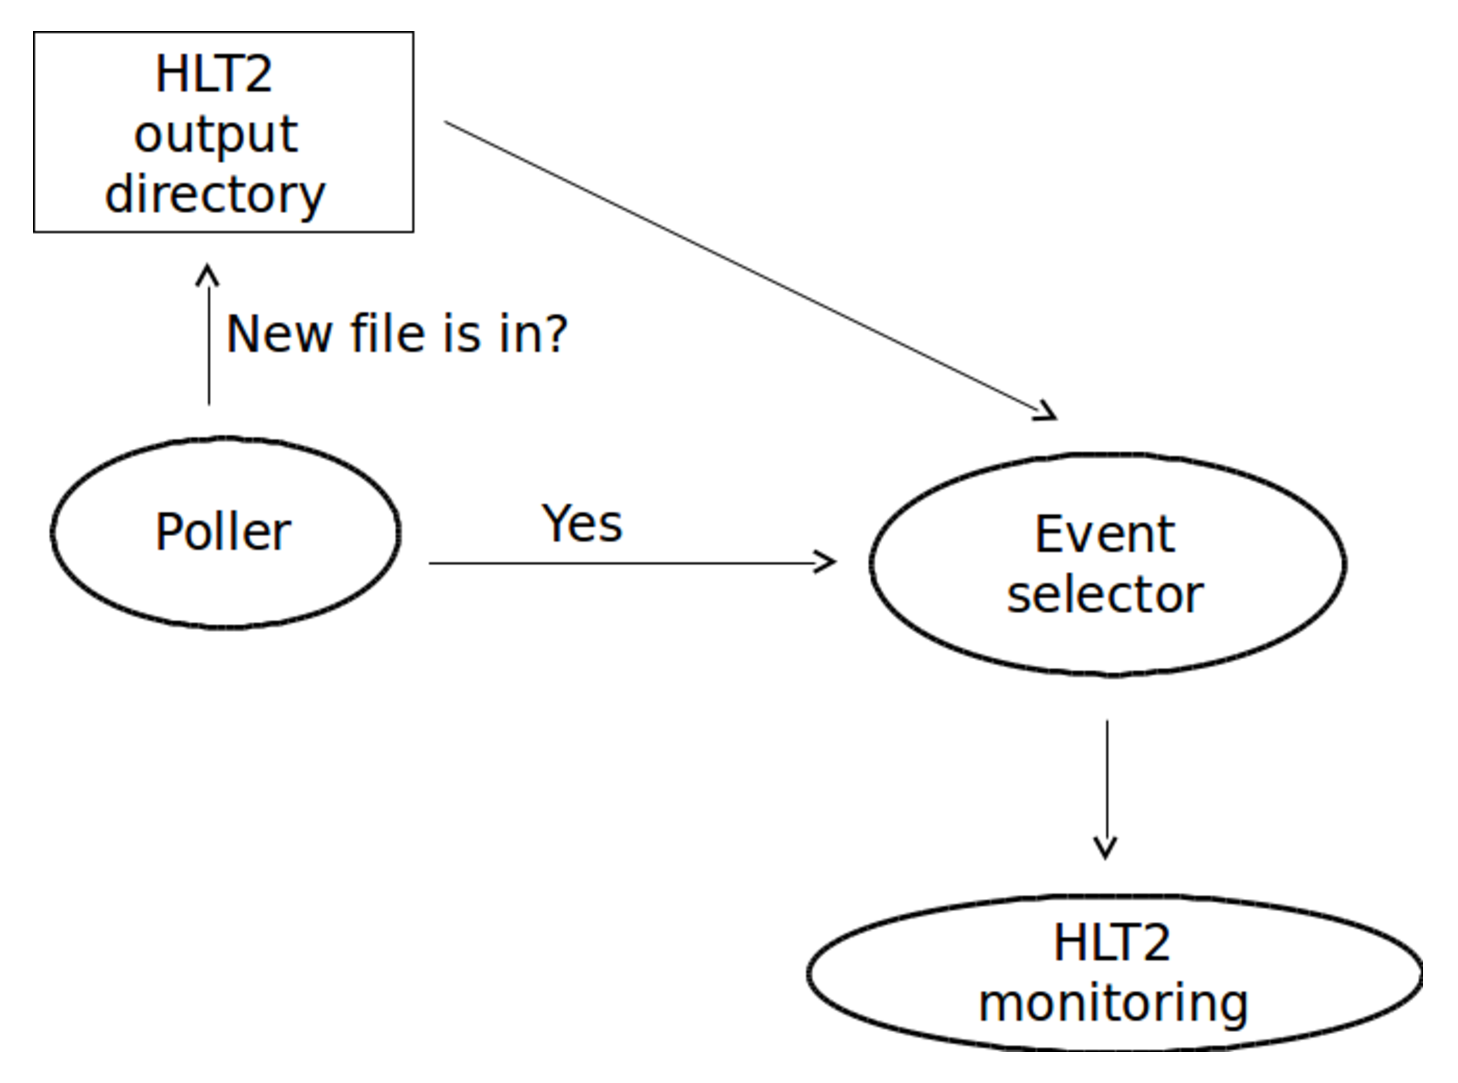
\includegraphics[height=\textheight,width=.8\textwidth, keepaspectratio=true]{figs/poller}}\par

\end{figure}


\subsubsection{\textbf{EventSelector}}
In the initialization of the \textit{EventSelector} pointers to other services are acquired. What we need to add to an \textit{EventSelector} to make it possible for it to use the poller are the following services, for which we acquire the necessary pointers : \textit{FilePoller}, \textit{HistogramDataSvc}, \textit{RootHistSvc} and \textit{HistogramPersistencySvc}. For details on the functionality of the latter three see \cite{mato1998gaudi}. Then we create the lock that will control the waiting/resuming of the \textit{EventSelector} during its interaction with the poller, and we initialize its value to zero, which means that at the beginning of its execution the \textit{EventSelector} will wait for input from the poller. Finally we initialize the counter \textit{m\_evtCount}, which counts the events read from a file and helps in deciding when the \textit{EventSelector} will go idle.
The \textit{start()}/\textit{stop()} methods are inherited from the base class \textit{Service}.\par
The \textit{EventLoopMgr} will use the \textit{EventSelector} to acquire the next event for processing -the \textit{next()} method of the \textit{EventSelector} gets called. After two initial checks regarding saving the histograms and updating the database (see later), the \textit{EventSelector} will check whether there is an input context (\textit{pCtxt != 0}).
If there is not, the \textit{EventSelector} will return StatusCode::FAILURE.\par
If there is an input context, we first have to check if this is the first connection (meaning \textit{m\_firstConnection == 0}) to an input file that the \textit{EventSelector} is trying to establish. Without this check we cannot safely call the \textit{receiveData()} method to read the next event.\par

\begin{itemize}
\item If it is the first connection the \textit{EventSelector} will finally go idle, that is it will connect to \textit{poller} and wait for an input file path (by calling the \textit{goIdle()} method).\par
\item If it is not the first connection, the \textit{EventSelector} will call \textit{receiveData()} to read the next event; if the call is successful the \textit{EventSelector} will increase the corresponding event counters and return StatusCode::SUCCESS. If it cannot read the next event (e.g. because there are no more events in the file), the \textit{EventSelector} will go idle after updating the database with the number of events it has read from the last input file and saving the histogram sets.\par
\end{itemize}
For the next calls of the  \textit{next()} method there are two checks preceding the input context check.\par
The first \textit{m\_maxNoEvt == m\_evtCount} checks whether we have reached the maximum number of events we want to read from one file. If we have, then the \textit{EventSelector} updates the database with the number of events so far read, resets the event counter, saves the histograms and then goes idle, waiting for the next file.If we want to read until the end of the file, we should set the \textit{m\_maxNoEvt} to -1.\par
%The second \textit{m\_EvtHisto} $\leq$  \textit{m\_totalEvt} checks whether we have read the necessary number of events to make a set of histograms. If yes, the event counter is reset to start counting again for the next set, we save the current set by calling \textit{saveHistos()} and then the \textit{EventSelector} goes idle.ONLY NEEDED IF WE WANT MORE THAN ONE HISTOFILES FROM THE SAME RUN\par
The second \textit{m\_runNum} $\neq$ \textit{m\_prevRun} checks whether the run has changed. If yes, it resets the event counter and changes the name of the file which will contain the next set of histograms.Then the \textit{EventSelector} continues reading events from the new file (and thus run). This check covers the case where the minimum number of events to produce a set of histograms is bigger then the events we have read from a file before changing it (e.g. covers the case of a very small run).\par
After having gone idle, the \textit{EventSelector} will wait at the corresponding lock (\textit{m\_suspendLock}) until the poller serves it with a file. In order for this to happen, the poller will call the \textit{alertSvc()} method of the \textit{EventSelector} passing as argument the file path to read from. This method before exiting will change the value of the \textit{m\_firstConnection} to 1, to signal that there has been at least one connection established.Next, it will get the current input context and update it with the new file path by calling \textit{resetCriteria()}.If the context update is successful, the \textit{EventSelector} reports back to the poller the \textit{successful opening} of the new file using \textit{statusReport()}. This means that the file and run will be added to the file database with a status flag of 0 : the file has been opened but we have not finished processing it.Then the poller will remove the \textit{EventSelector} from the waiting spot, extract the new run number from the file path and generate accordingly the new histogram set name.It will finally resume the operation of the \textit{EventSelector}, which will continue from the point where the last call of \textit{goIdle()} was made.\par
At the end of the execution cycle, the inherited \textit{stop()} method is called and then the \textit{finalize()}. In the \textit{finalize()} method we reset the counters, remove the acquired interfaces by setting the pointers to them to 0 and we delete the wait/resume lock of the \textit{EventSelector}.

\subsubsection{\textbf{Details about Poller methods and member variables}}

\begin{itemize}

\item std::string m\_scanDirectory : this is the directory that the poller will check periodically for files, which will then distribute to the listeners\par
\item int m\_alrmTime : the time interval between two successive pollings\par
\item std::deque$<$std:string$>$ m\_fileNames : the list of the file paths that were found in the scanned directory during the last polling.\par 
\bigskip\noindent
The \textit{std::deque} container was chosen for the above list as it implements a First In First Out structure, which is what we want especially for the listeners : the poller should serve first the listener who asked first for a new file. Furthermore, a  \textit{std::deque} performs better than a vector at the removal of its first element and grows more efficiently in size.\par
\bigskip\noindent
\item mutable $<$IAlertSvc*$>$ m\_EvtSelector : the listener waiting for input from the poller. It is kept in the form of a pointer to its \textit{IAlertSvc} interface.\par
\item sqlite3* m\_FileInfo : the handler of the database keeping the file/run information.\par
\bigskip\noindent
The necessary accesor methods for the above private member variables are provided : \textit{addTofileNames,remFromfileNames}.\par
Some more implementation details about methods that were mentioned in the workflow:\par
\item StatusCode poller(const std::string scan\_path) : This is the method that performs the polling.It uses \textit{readdir\_r} to scan the directory. If it finds a file, it adds it to the file list whereas if it finds another directory it calls itself recursively to scan it (apart from the current (\textit{\"~.\"}) and previous  (\textit{\"~..\"}) directories).\par
\item StatusCode statusReport(StatusCode status,const std::string file) : This method gives feedback to the poller about the \textit{opening} of the file from the \textit{EventSelector}.If the opening was unsuccessful the method \textit{issueAlarm()} is called, which inserts an error record into the database containing the file name, the run number and the value of -1 in the event counter and status flag.If the opening was succesful, we insert the file name into the database, marking it as unprocessed/currently in process (\textit{StatusFlag == 0}), using the method \textit{markBookKept()}.\par
\item const StatusCode issueAlarm(const std::string& msg) : In case the \textit{EventSelector} does not manage to open a file from the path it has received, it is not enough to print a message reporting it. This method provides support for this case by adding an entry in the database with the name of the file that failed to be opened, the run it belongs to and the value of -1 in the \textit{StatusFlag} and '\textit{TotalEvents} fields.\par
\item StatusCode isBookKept(const std::string file) : It checks if the file passed as its argument is in the database with \textit{StatusFlag == 0},i.e. it is currently being processed.\par
\item StatusCode isProcessed(const std::string file) : It checks if the file passed as its argument is in the database with \textit{StatusFlag == 1}.\par
\item StatusCode updateStatus(const std::string file, int events) : It updates the record in the database which corresponds to the file passed as argument, with the number of events passed as the second argument.\par

\end{itemize}


\subsubsection{\textbf{Details about EventSelector methods and member variables}}
\begin{itemize}
\item std::string m\_HistoDirectory : this is the output directory for the histogram sets saved by the poller\par
\item StatusCode goIdle() const : This method is called for the transition of the \textit{EventSelector} from a running to an idle state.It first sets the \textit{m\_isWaiting} flag to true. Then the \textit{EventSelector} is added to the listener spot of the poller by calling \textit{addListener()}.If the registration to the poller is successful, the \textit{EventSelector} waits at the \textit{m\_suspendLock}. If it cannot acquire the waiting lock it removes itself from the listener spot by calling \textit{remListener()}. Either after its removal or when it resumes execution after having successfully waited, the \textit{m\_isWaiting} flag is set to false.\par

\item StatusCode saveHistos() const : This method is responsible for saving the histogram sets. Normally these steps would be carried out when the event loop would have finished, but since the poller will be constantly running this will happen only at the end of the processing of all runs. The need to save the sets at the end of each run called for the integration of this code here. The histograms are traversed, conversed to their permanent representation (e.g. ROOT) and saved. In order to create a new file for each saveset and not overwrite the same saveset again and again, the histograms must be reset and a new file name has to be selected for the histogram file. Whenever we have to save the histograms (that is either when we have reached the necessary number of events or when the run has changed), the conversion service (\textit{m\_RootHistSvc}) is stopped and finalised. The methods \textit{sysStop()} and \textit{sysFinalize()} are called instead of the  \textit{stop()} and \textit{finalize()} to avoid execution errors because these methods change the state of the machine according to their function from running to configure.If a new file is going to be opened next, that is if a new run is going to be processed, the name of the histogram file is changed. It is in this method (\textit{setNewHistosName()}) that we reintialize and restart the conversion service.


\end{itemize}


%\section{How to run and test Poller}\label{sec:HowTo}
%\subsection{\textbf{Prerequisites}}
%This section will give some instructions on how to run the polling service. It takes for granted that the \textit{EventSelector} used will have been modified to use the poller, as described above.\par
%The \textit{OnlineFileSelector} package should be in the same \textit{VanDerMeer} project directory, or the monitoring scripts should be able to "see" it by including it in the \textit{requirements} file of their \textit{cmt} directory.\par.\subsection{\textbf{Running}}
%In order to run the \textit{poller}, an instance of it and of a modified \textit{EventSelector} should be instantiated and its variables initialized (scan directory, alarm timer). Next follow the code excerpts of a testing python script that do the job : \par

%\begin{itemize}
%\item Import : from Configurables import ( \par
%             \hspace{20mm} LHCb\_MDFOnlineEvtSelector,\par
%             \hspace{20mm} LHCb\_FilePoller,\par
%                           )  \par
%\item Initial output file : HistogramPersistencySvc().OutputFile = "testPol.root" \par
%\item Poller instantiation and setting parameters : \par
%                 \hspace{20mm}poller = LHCb\_FilePoller('Poller')\par
%                 \hspace{20mm}appMgr.ExtSvc.append(poller)\par
%                 \hspace{19mm}poller.scanDirectory = "/daqarea/lhcb/data/2014/RAW/FULL/LHCb1/TEST"  \par
%                 \hspace{20mm}poller.alarmTime = 3\par
%                 \hspace{20mm}poller.DbName = "./OnlineFileProcessing.db"\par

%\item EventSelector instantiation and setting parameters : \par
%               \hspace{17mm}selector = LHCb\_MDFOnlineEvtSelector('EventSelector')\par
%               \hspace{20mm}appMgr.ExtSvc.append(selector)\par
%               \hspace{20mm}selector.MaxNoEvents = 50000;\par
%               \hspace{20mm}selector.PrintFreq = 10000\par
%               \hspace{20mm}selector.HistogramFile = "testPollerPr.root"\par
%               \hspace{20mm}selector.EvtsForHist = 30000 \par
%               \hspace{20mm}selector.SaveHistoDir = "./HLT2/" \par

%\end{itemize}

%Next follows a typical python script running the poller and producing the same histograms as \textit{HltMassMonitor} program.The histograms will be saved in thedirectory specified in the script.The following procedure should be executed to run the script (provided the following packages are inside \textit{VanDerMeer v6r1}:\textit{OnlineFileSelector, Monitor/HltMonitor, Monitor/CommonMonitor} ):
%\begin{itemize}
%\item run the \textit{SetupVanDerMeer\_v6r1.sh} script, which is inside \textit{Monitor/CommonMonitor/job/}
%\item compile the \textit{OnlineFileSelector} package by running \textit{cmt make} in the \textit{cmt} directory of the package \textit{OnlineFileSelector}
%\item execute (\textit{source}) the setup script in the \textit{cmt} directory of \textit{HltMonitor}
%\item compile the \textit{HltMonitor} by running \textit{cmt make} in its \textit{cmt} directory
%\item run \textit{gaudirun.py testPoller.py} inside \textit{HltMonitor/scripts/}

%\end{itemize}

%\begin{figure}
%\caption{\textit{Sample script}}
%\centering
%\fbox{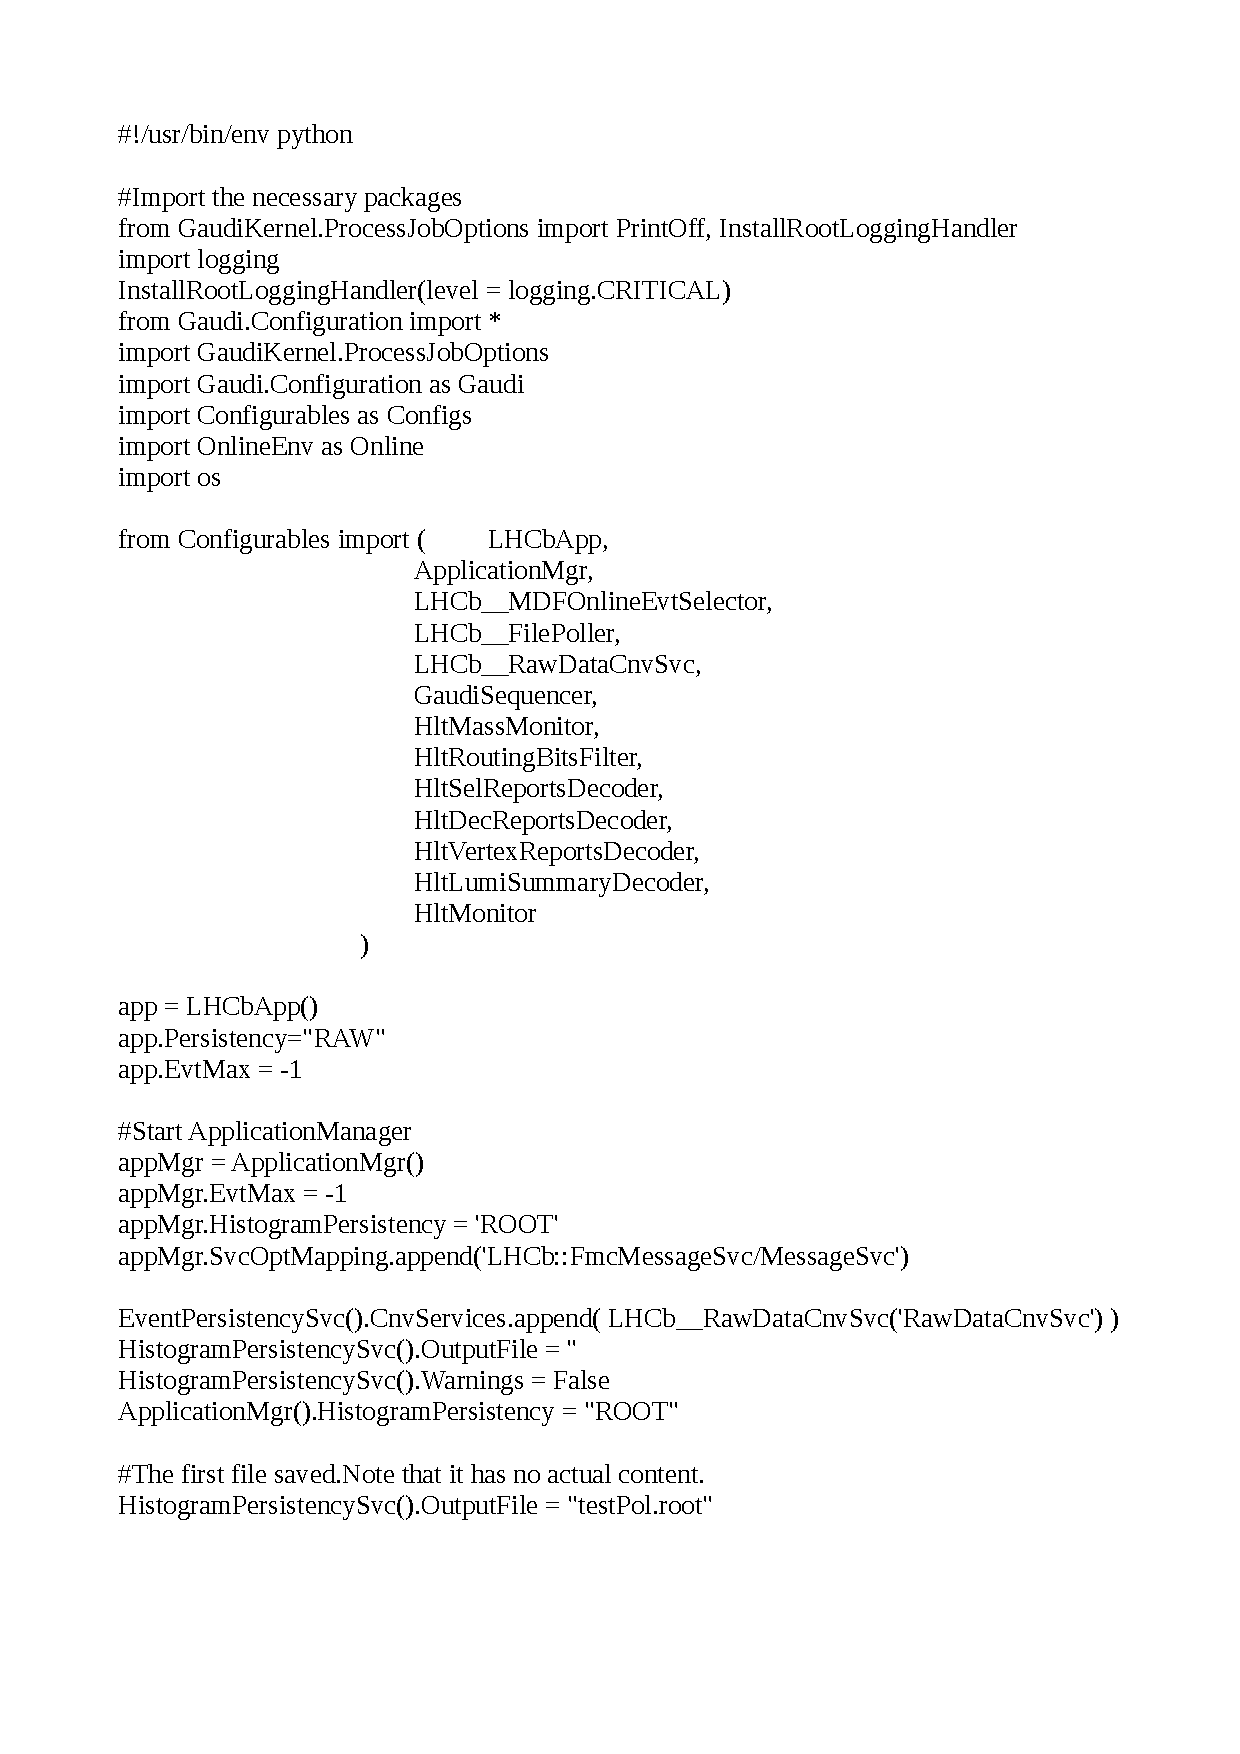
\includegraphics[height=\textheight,width=\textwidth, keepaspectratio=true]{figs/testpoller2}}\par
%\end{figure}\par

%\begin{figure}
%\caption{\textit{Sample script}}
%\centering
%\fbox{\includegraphics[height=\textheight,width=\textwidth, keepaspectratio=true,page=2]{figs/testpoller2}}\par
%\end{figure}\par

%\begin{figure}
%\caption{\textit{Sample script}}
%\centering
%\fbox{\includegraphics[height=\textheight,width=\textwidth, keepaspectratio=true,page=3]{figs/testpoller2}}\par
%\end{figure}\par

\section{Implementation and workflow of the FilePollerNFiles}\label{sec:ImplementationN}

\subsection{\textbf{Introduction}}
In addition to the simple poller described above, the following part describes the functionality of the \textit{FilePollerNFiles}, which does not send a run for processing unless there are N files available for reading from that run.To support this functionality we had to add a table in the database, which holds the run number and the number of available files that belong to that run.As soon as this number is greater than or equal to N, we start distributing the files to the event selector.\par

\subsection{\textbf{Dependencies}}
--No extra dependencies--

\subsection{\textbf{Workflow}}
The ApplicationManager initializes the required services (for details see ADD \cite{mato1998gaudi}), among them the \textit{Poller} and the \textit{EventSelector}.\par

\subsubsection{\textbf{Poller}}
The initialization is completed by calling the \textit{initialize()} method of the poller, which first connects to the database where it will store the run-related information (or creates a new database if one does not exist). The execution continues with the \textit{start()} method, which sets the timer and starts the countdown until the next polling.\par
When the timer expires, the \textit{timerHandler()} method gets called. It will first call the \textit{poller()} method which takes as argument the directory to be scanned for new files. Then it will start distributing the file paths to the listener and it will stop when there are no more files to distribute.The process for distributing the files is as follows:~First the file path is removed (\textit{remFromfileNames()}) from the list of available file paths, which was filled during the last polling period.From that path we extract the run number (\textit{getRunFileNumber()}) which we will use to check whether we have to process the run. First we acquire the counter of the files we have yet to read from this run.If the counter is -1, we do not need to read any more files from this particular run, so we 'free' the \textit{EventSelector} that handled it (\textit{clearRun(run)}), that is, the event selector is now able to be assigned a different run; then we skip the current file and move on to the next one.\par
Next, using the file name we check :\par
\begin{itemize}
\item if we had tried to open the file but we encountered an error and the file should not be tried again (\textit{isDefect()}),\par
\item if the file has already been processed (\textit{isProcessed()}), or\par
\item if we have already opened it and is currently being processed (\textit{inProcess()})\par
\end{itemize}
If one of the above mentioned cases occurs we skip the processing of the current file.All these methods check the \textit{StatusFlag} of the corresponding file, which has four possible values :\par
\begin{itemize}
\item -1~:~ erroneous file\par
\item 0~:~ the file has just been inserted in the database\par
\item 1~:~ the file has already been processed\par
\item 2~:~ the file is currently being processed\par
\end{itemize}
If none of the above methods returns \textit{StatusCode::SUCCESS} we check whether we have available the minimum number of files to start processing the run.If that is the case, we mark the run as ready to be processed. A file whose run is 'ready' to be processed is then passed on to the listener.\par
When the distribution of the files is over, we empty the vector holding the remaining file paths (if any) and the timer is reset.\par
At the end of the execution cycle, the \textit{stop()} method is called which stops the service and the countdown of the timer. It is followed by a call to the \textit{finalize()} method which closes the connection to the file database.\par


\subsubsection{\textbf{EventSelector}}
In the initialization of the \textit{EventSelector} pointers to other services are acquired. What we need to add to an \textit{EventSelector} to make it possible for it to use the poller are the following services, for which we acquire the necessary pointers : \textit{FilePoller}, \textit{HistogramDataSvc}, \textit{RootHistSvc} and \textit{HistogramPersistencySvc}. For details on the functionality of the latter three see \cite{mato1998gaudi}. Then we create the lock that will control the waiting/resuming of the \textit{EventSelector} during its interaction with the poller, and we initialize its value to zero, which means that at the beginning of its execution the \textit{EventSelector} will wait for input from the poller. Finally we initialize the counter \textit{m\_evtCount}, which counts the events read from a file and helps in deciding when the \textit{EventSelector} will go idle.
The \textit{start()}/\textit{stop()} methods are inherited from the base class \textit{Service}.\par
The \textit{EventLoopMgr} will use the \textit{EventSelector} to acquire the next event for processing -the \textit{next()} method of the \textit{EventSelector} gets called. After two initial checks regarding saving the histograms and updating the database (see later), the \textit{EventSelector} will check whether there is an input context (\textit{pCtxt != 0}).
If there is not, the \textit{EventSelector} will return StatusCode::FAILURE.\par
If there is an input context, we first have to check if this is the first connection (meaning \textit{m\_firstConnection == 0}) to an input file that the \textit{EventSelector} is trying to establish. Without this check we cannot safely call the \textit{receiveData()} method to read the next event.\par

\begin{itemize}
\item If it is the first connection the \textit{EventSelector} will finally go idle, that is it will add itself to the listener spot of the \textit{poller} and wait for an input file path (by calling the \textit{goIdle()} method).\par
\item If it is not the first connection, the \textit{EventSelector} will call \textit{receiveData()} to read the next event; if the call is successful the \textit{EventSelector} will increase the corresponding event counters and return StatusCode::SUCCESS. If it cannot read the next event (e.g. because there are no more events in the file), the \textit{EventSelector} will go idle after updating the database with the number of events it has read from the last input file.If the file was the last one available from the particular run that is currently being processed, the histogram sets will be saved as well.\par
\end{itemize}
For the next calls of the  \textit{next()} method there are two checks preceding the input context check.\par
The first \textit{m\_maxNoEvt == m\_evtCount} checks whether we have reached the maximum number of events we want to read from one run. If we have, then the \textit{EventSelector} updates the database with the number of events read from the last file, saves the histograms and then goes idle, waiting for the next file/run.If we want to read until the end of every file of the run we are processing, we should set the \textit{m\_maxNoEvt} to -1.\par
%The second \textit{m\_EvtHisto} $\leq$  \textit{m\_totalEvt} checks whether we have read the necessary number of events to make a set of histograms. If yes, the event counter is reset to start counting again for the next set, we save the current set by calling \textit{saveHistos()} and then the \textit{EventSelector} goes idle.ONLY NEEDED IF WE WANT MORE THAN ONE HISTOFILES FROM THE SAME RUN\par
The second \textit{m\_runNum} $\neq$ \textit{m\_prevRun} checks whether the run has changed. If yes, it resets the event counter and changes the name of the file which will contain the next set of histograms.Then the \textit{EventSelector} continues reading events from the new run.\par
After having gone idle, the \textit{EventSelector} will wait at the corresponding lock (\textit{m\_suspendLock}) until the poller serves it with a file. In order for this to happen, the poller will call the \textit{alertSvc()} method of the \textit{EventSelector} passing as argument the file path to read from. This method before exiting will change the value of the \textit{m\_firstConnection} to 1, to signal that there has been at least one connection established.Next, it will get the current input context and update it with the new file path by calling \textit{resetCriteria()}.If the context update is successful, the \textit{EventSelector} reports back to the poller the \textit{successful opening} of the new file using \textit{statusReport()}. This means that the file and run will be updated in the file database with a status flag of 2 : the file has been opened but we have not finished processing it.Then the poller will remove the \textit{EventSelector} from the listener spot, extract the new run number from the file path and generate accordingly the new histogram set name.It will finally resume the operation of the \textit{EventSelector}, which will continue from the point where the last call of \textit{goIdle()} was made.\par
At the end of the execution cycle, the inherited \textit{stop()} method is called and then the \textit{finalize()}. In the \textit{finalize()} method we reset the counters, remove the acquired interfaces by setting the pointers to them to 0 and we delete the wait/resume lock of the \textit{EventSelector}.

\subsubsection{\textbf{Details about Poller methods and member variables}}

\begin{itemize}

\item std::string m\_minFileNum : this is the minimum number of files of a run that should be available in order to start processing the corresponding run.There may be more files of the run available but we will try to process \textit{m\_minFileNum} number of files.\par 
\item std::string m\_scanDirectory : this is the directory that the poller will check periodically for files, which will then distribute to the listeners\par
\item int m\_alrmTime : the time interval between two successive pollings\par
\item std::deque$<$std:string$>$ m\_fileNames : the list of the file paths that were found in the scanned directory during the last polling.\par 
\bigskip\noindent
The \textit{std::deque} container was chosen for the above list as it implements a First In First Out structure, which is what we want especially for the listeners : the poller should serve first the listener who asked first for a new file. Furthermore, a  \textit{std::deque} performs better than a vector at the removal of its first element and grows more efficiently in size.\par
\bigskip\noindent
\item mutable $<$IAlertSvc*$>$ m\_EvtSelector : the listener waiting for input from the poller. It is kept in the form of a pointer to its \textit{IAlertSvc} interface.\par
\item sqlite3* m\_FileInfo : the handler of the database keeping the file/run information.\par
\bigskip\noindent
The necessary accesor methods for the above private member variables are provided : \textit{addTofileNames,remFromfileNames}.\par
Some more implementation details about methods that were mentioned in the workflow:\par

\item StatusCode poller(const std::string scan\_path) : In this implementation of the polling function we have added the functionality of inserting a run in the database or increasing the run's file counter.When we scan a file in the directory, we check the buffer to make sure we have not buffered it before (if (find( m\_fileNames.begin(),  m\_fileNames.end(),n\_path) ==  m\_fileNames.end())).If we have not, then it is added to the buffer (\textit{m\_fileNames}).For this version of the poller, we proceed to check if the file is in the files table of the database and if it is not (\textit{StatusCode::FAILURE == isBookKept(file\_regexp)}) we insert it in the table \textit{FileRecords} with the \textit{StatusFlag} set to zero.Then we check if the run (that the file belongs to) is in the run database:~if not, we insert it and if it is, and we still need to process the run (\textit{if (-1 != getCounter(run))}), we increase the file counter.\par

\item StatusCode statusReport(StatusCode status,const std::string file) : This method gives feedback to the poller about the \textit{opening} of the file from the \textit{EventSelector}.If the opening was unsuccessful the method \textit{issueAlarm()} is called, which inserts an error record into the database containing the file name, the run number and the value of -1 in the event counter and status flag. If the opening was succesful, we insert the file name into the database, marking it as currently in process (\textit{StatusFlag == 2}), using the method \textit{SetInProcess()}.\par

\item const StatusCode issueAlarm(const std::string& msg) : In case the \textit{EventSelector} does not manage to open a file from the path it has received, it is not enough to print a message reporting it. This method provides support for this case by adding an entry in the database with the name of the file that failed to be opened, the run it belongs to and the value of -1 in the \textit{StatusFlag} and '\textit{TotalEvents} fields.Since such a file will not be processed again, it also decreases the counter of available files of the particular run. If there are no more files available it also frees the event selector which was assigned to that run (\textit{clearRun()}).\par

\item StatusCode isBookKept(const std::string file) : It checks if the file passed as its argument is in the database with \textit{StatusFlag == 0},i.e. it has just been inserted into the database..\par

\item StatusCode isProcessed(const std::string file) : It checks if the file passed as its argument is in the database with \textit{StatusFlag == 1}.\par

\item StatusCode updateStatus(const std::string file, int events) : It updates the record in the database which corresponds to the file passed as argument, with the number of events passed as the second argument.It also decreases the counter of available files of the particular run, since this method is called when we have finished processing one file. If it was the last available file, we mark the run as processed,i.e. its file counter is set to -1.\par

\item StatusCode insertRun(const std::string run) : This method inserts the run into the corresponding table and initializes the file counter to 0.\par

\item StatusCode existsRun(const std::string run) : This method checks whether the run passed as argument is present in the database.\par

\item StatusCode distributeFile(const std::string run, const std::string path\_name) : This method takes care of the distribution of a file to the event selector. If the current run is empty or is the same as the run that \textit{path\_ name} belongs to, we forward the file to the event selector. If it is not,then we return successfully as it is implied that the event selector is busy handling a different run.\par
\end{itemize}


\subsubsection{\textbf{Details about EventSelector methods and member variables}}
\begin{itemize}
\item std::string m\_HistoDirectory : this is the output directory for the histogram sets saved by the poller\par
\item StatusCode goIdle() const : This method is called for the transition of the \textit{EventSelector} from a running to an idle state.It first sets the \textit{m\_isWaiting} flag to true. Then the \textit{EventSelector} is added to the listener spot of the poller by calling \textit{addListener()}.If the registration to the poller is successful, the \textit{EventSelector} waits at the \textit{m\_suspendLock}. If it cannot acquire the waiting lock it removes itself from the listener spot by calling \textit{remListener()}. Either after the removal from the list or when it resumes execution after having successfully waited, the \textit{m\_isWaiting} flag is set to false.\par

\item StatusCode saveHistos() const : This method is responsible for saving the histogram sets. Normally these steps would be carried out when the event loop would have finished, but since the poller will be constantly running this will happen only at the end of the processing of all runs. The need to save the sets at the end of each run called for the integration of this code here. The histograms are traversed, conversed to their permanent representation (e.g. ROOT) and saved. In order to create a new file for each saveset and not overwrite the same saveset again and again, the histograms must be reset and a new file name has to be selected for the histogram file. Whenever we have to save the histograms (that is either when we have reached the necessary number of events or when the run has changed), the conversion service (\textit{m\_RootHistSvc}) is stopped and finalised. The methods \textit{sysStop()} and \textit{sysFinalize()} are called instead of the  \textit{stop()} and \textit{finalize()} to avoid execution errors because these methods change the state of the machine according to their function from running to configure.If a new file is going to be opened next, that is if a new run is going to be processed, the name of the histogram file is changed. It is in this method (\textit{setNewHistosName()}) that we reintialize and restart the conversion service.\par
NOTE: The first histogram file containing actual content will be the one with the correct name (with respect to the run the histograms come from) and not whichever name is set in the python configuration script under \textit{HistogramPersistencySvc().OutputFile}.\par


\end{itemize}


\section{How to run and test Poller}\label{sec:HowTo}
\subsection{\textbf{Prerequisites}}
This section will give some instructions on how to run the polling service. It takes for granted that the \textit{EventSelector} used will have been modified to use the poller, as described above.\par
The \textit{OnlineFileSelector} package should be in the same \textit{VanDerMeer} project directory, or the monitoring scripts should be able to "see" it by including it in the \textit{requirements} file of their \textit{cmt} directory.\par.\subsection{\textbf{Running}}
In order to run the \textit{poller}, an instance of it and of a modified \textit{EventSelector} should be instantiated and its variables initialized (scan directory, alarm timer). Next follow the code excerpts of a testing python script that do the job : \par

\begin{itemize}
\item Import : from Configurables import ( \par
              \hspace{20mm} LHCb\_MDFOnlineEvtSelectorNFiles,\par
              \hspace{20mm} LHCb\_FilePollerNFiles,\par
                            )  \par
\item Initial output file : HistogramPersistencySvc().OutputFile = "" \par
\item Poller instantiation and setting parameters : \par
                 \hspace{20mm}poller = LHCb\_FilePollerNFiles('Poller')\par
                 \hspace{20mm}appMgr.ExtSvc.append(poller)\par
                 \hspace{19mm}poller.scanDirectory = "/daqarea/lhcb/data/2014/RAW/FULL/LHCb1/TEST"  \par
                 \hspace{20mm}poller.MinimumFileNum = 2\par
                 \hspace{20mm}poller.alarmTime = 3\par
                 \hspace{20mm}poller.DbName = "./OnlineFileProcessing.db"\par

\item EventSelector instantiation and setting parameters : \par
               \hspace{17mm}selector = LHCb\_MDFOnlineEvtSelectorNFiles('EventSelector')\par
               \hspace{20mm}appMgr.ExtSvc.append(selector)\par
               \hspace{20mm}selector.MaxNoEvents = 50000;\par
               \hspace{20mm}selector.PrintFreq = 10000\par
               \hspace{20mm}selector.HistogramFile = ""\par
               \hspace{20mm}selector.EvtsForHist = 30000 \par
               \hspace{20mm}selector.SaveHistoDir = "./HLT2/" \par

\end{itemize}

Next follows a typical python script running the poller and producing the same histograms as \textit{HltMassMonitor} program.The histograms will be saved in the directory specified in the script.The following procedure should be executed to run the script (provided the following packages are inside \textit{VanDerMeer v6r1}:\textit{OnlineFileSelector, Monitor/HltMonitor, Monitor/CommonMonitor} ):
\begin{itemize}
\item run the \textit{SetupVanDerMeer\_v6r1.sh} script, which is inside \textit{Monitor/CommonMonitor/job/}
\item compile the \textit{OnlineFileSelector} package by running \textit{cmt make} in the \textit{cmt} directory of the package \textit{OnlineFileSelector}
\item execute (\textit{source}) the setup script in the \textit{cmt} directory of \textit{HltMonitor}
\item compile the \textit{HltMonitor} by running \textit{cmt make} in its \textit{cmt} directory
\item run \textit{gaudirun.py testPoller.py} inside \textit{HltMonitor/scripts/}

\end{itemize}

\begin{figure}
\caption{\textit{Sample script}}
\centering
\fbox{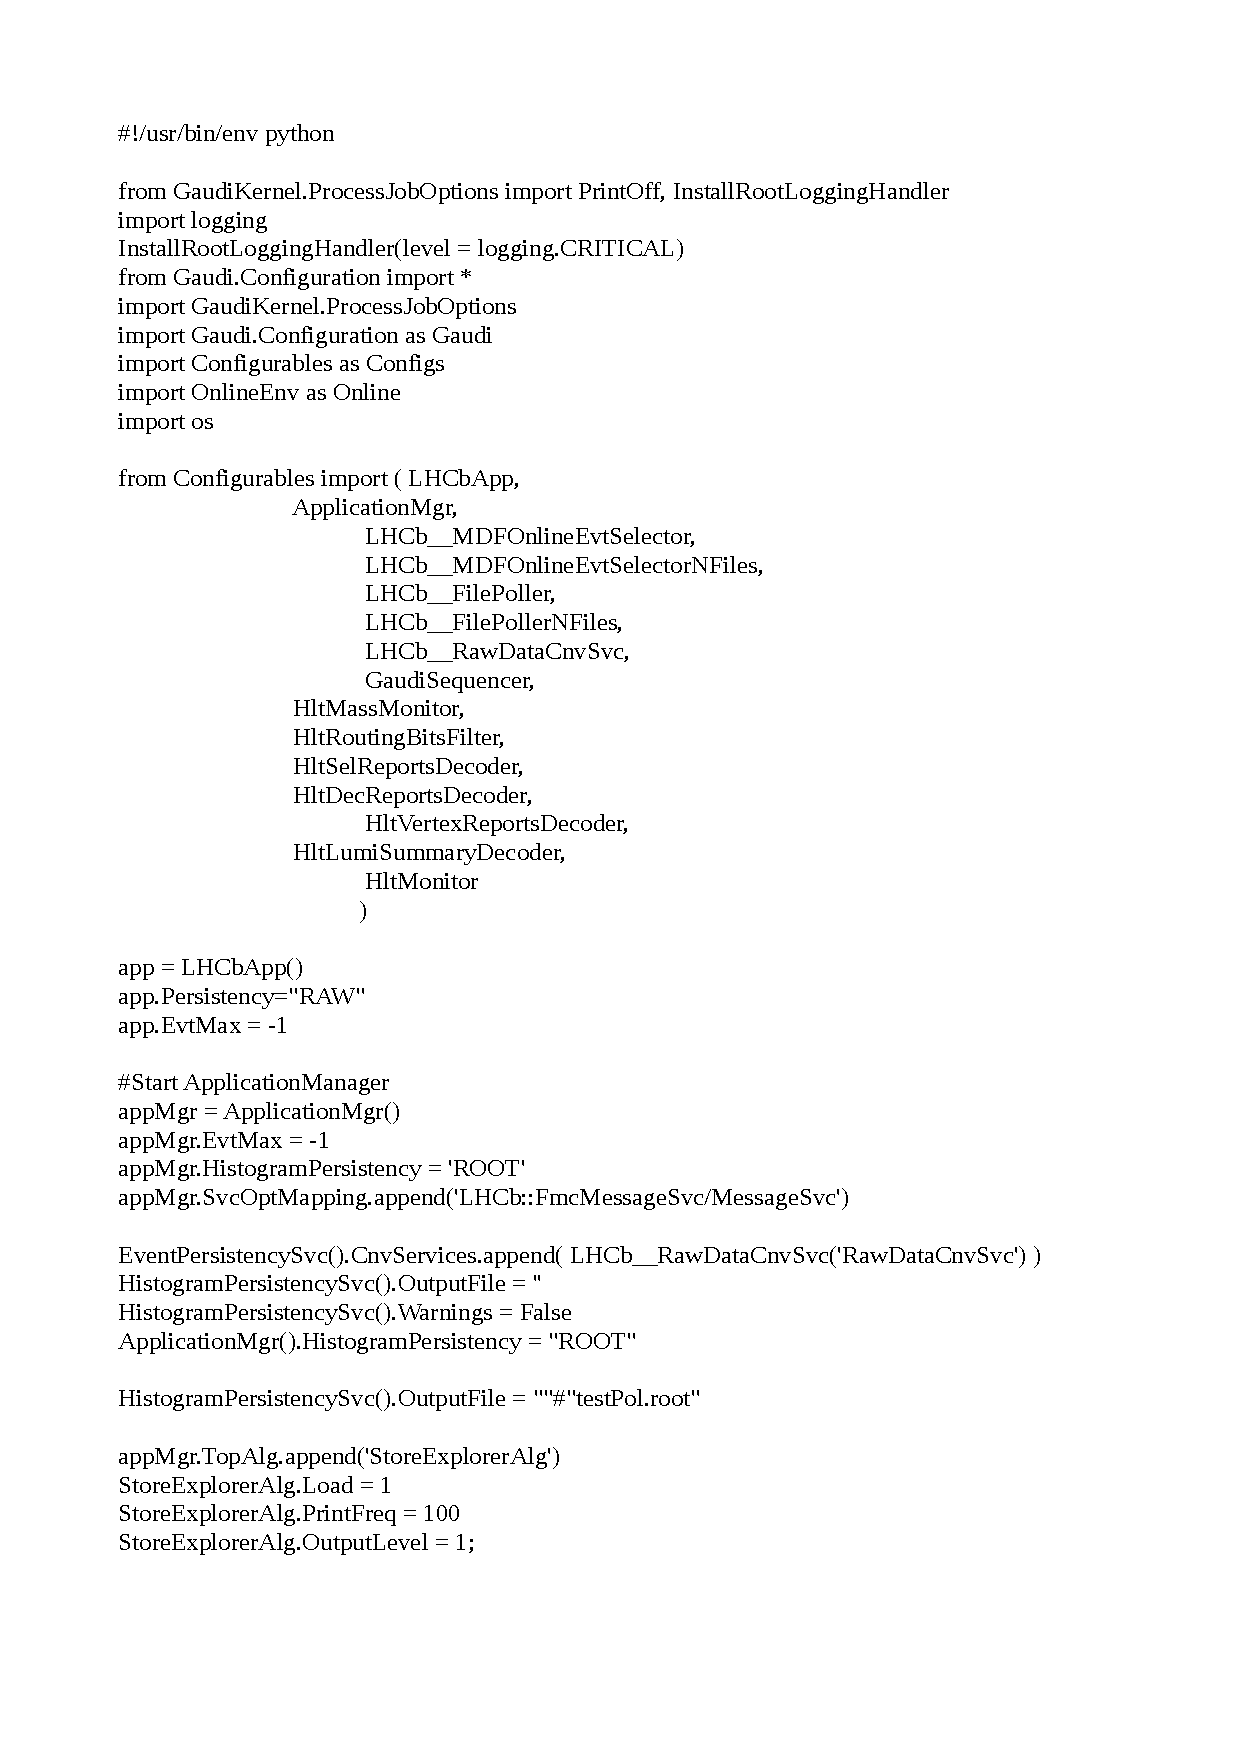
\includegraphics[height=\textheight,width=\textwidth, keepaspectratio=true]{figs/testpoller3}}\par
\end{figure}\par

\begin{figure}
\caption{\textit{Sample script}}
\centering
\fbox{\includegraphics[height=\textheight,width=\textwidth, keepaspectratio=true,page=2]{figs/testpoller3}}\par
\end{figure}\par

Note: Make sure to compile and instantiate the poller and the corresponding event selector : FilePoller/MDFEvtSelector or FilePollerNFiles/MDFEvtSelectorNFiles.\par

\newpage

%\begin{figure}
%\caption{\textit{Sample script}}
%\centering
%\fbox{\includegraphics[height=\textheight,width=\textwidth, keepaspectratio=true,page=3]{figs/testpoller2}}\par
%\end{figure}\par

\section{HLT monitoring}\label{sec:Hlt}
A brief introduction to the monitoring process and a description of the monitoring programs is given in this section. The main monitoring software is in \textit{HltMonitor.cpp} (for HLT 1) and \textit{HltMassMonitor.cpp} (for HLT 2).\par

\subsection{\textbf{Online data monitoring}\cite{Callot:1177133}}
The front-end readout electronics of the detector send the data collected during the collisions to the HLT farm nodes, where it is decided whether the event will be accepted.Events that are accepted from the HLT algorithms are sent to the storage and the GRID for further analysis.A fraction of these events is directed to the monitoring farm, which executes tasks which monitor the detector response in order to ensure data integrity and to detect malfunctioning components early (\textit{see fig.4}).\par
Each task in the monitoring farm creates its own set of monitoring information.This implies that all data are distributed over all tasks and the monitoring information is not appropriate for analysis; first it must be collected and summed (\textit{see fig.5}).\par
Dedicated tasks (\textit{Adders}) sum the corresponding items published by a set of monitoring tasks and then they publish the summed information. Monitoring information is pushed to these tasks at regular intervals to obtain coherent snapshots of the published information. Such snapshots are created by the monitoring 
applications at regular intervals during the data taking activity and at a run change.In the event of irregularities an alarm is raised and displayed by the 
experiment control system. A program called the Presenter allows the user to view and process the summed monitoring information.\par

\begin{figure}
\caption{\textit{The hardware layout.Tell1 are the readout boards.}\cite{Callot:1177133}}
\centering
\fbox{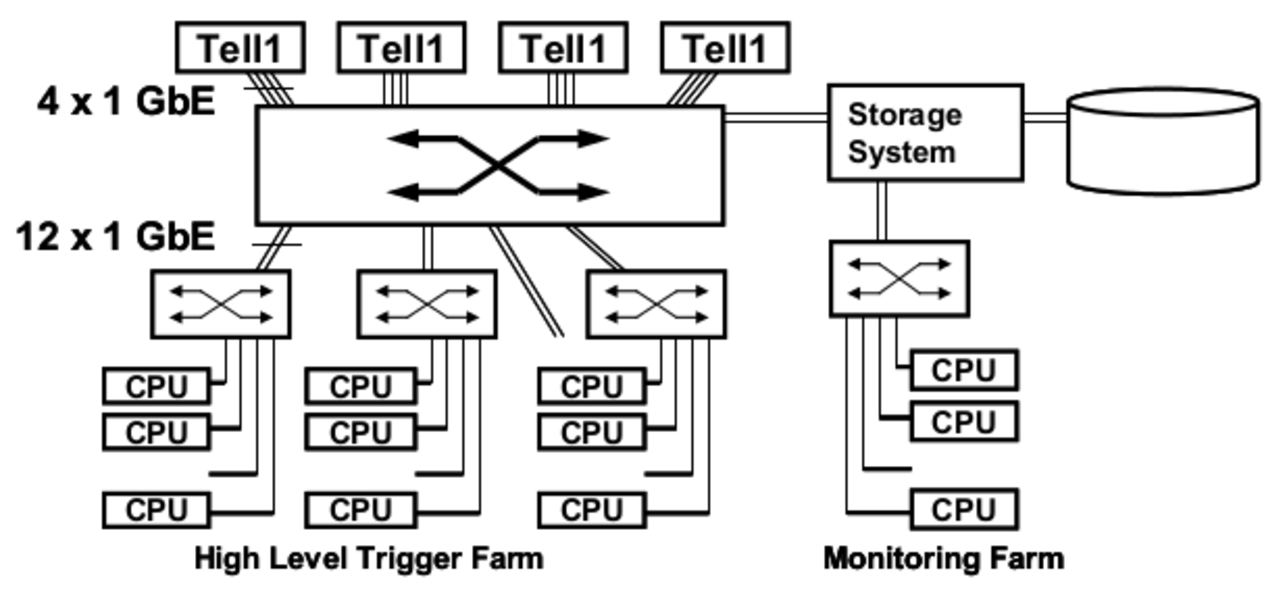
\includegraphics[height=\textheight,width=.8\textwidth, keepaspectratio=true]{figs/monitorHardWare}}\par
\end{figure}

\begin{figure}
\caption{\textit{The flow of the monitoring information.}\cite{Callot:1177133}}
\centering
\fbox{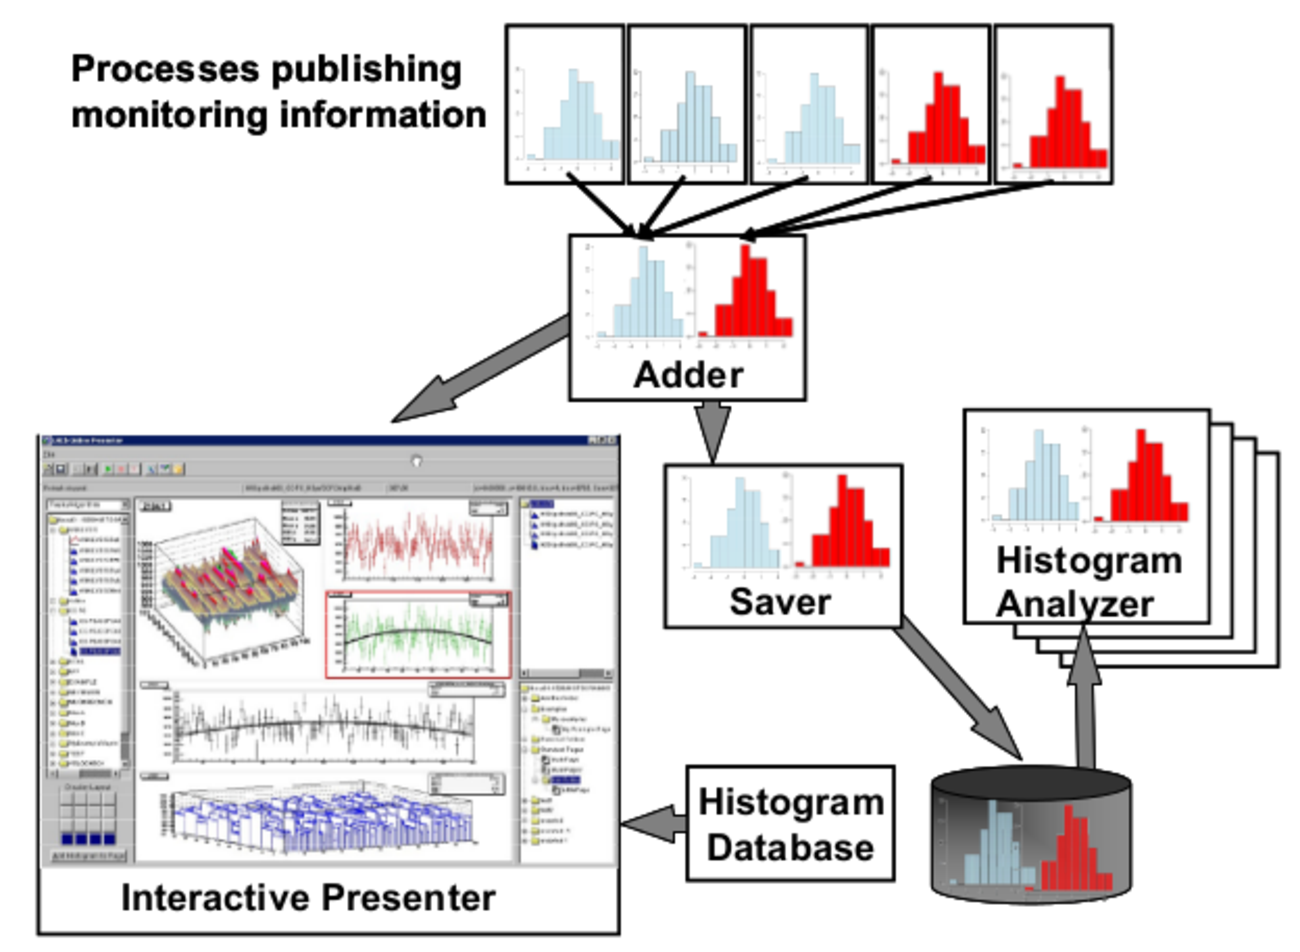
\includegraphics[height=\textheight,width=.8\textwidth, keepaspectratio=true]{figs/monitorInfoFlow}}\par
\end{figure}


\subsection{\textbf{HLT1 monitoring}}

\subsubsection{\textbf{HltMonitor.cpp}}
\subsubsection{\textbf{Introduction}}
The program flow follows the basic pattern of execution inside \textit{Gaudi}~:
initialization (\textit{initialize()}), execution ({\textit{execute()}}) and finalization ({\textit{finalize()}}). The execution method invokes all the actual monitoring methods.\par
First, some key objects present in the monitoring code will be presented and the description of the program flow will follow.\par
The first part of the documentation refers to the source file \textit{HltMonitor.cpp} found in \textit{VanDerMeer\_v6r1/Monitor/HltMonitor/src}.

\subsubsection{\textbf{RawEvent,routing bits and other key objects in monitoring}}

The \textit{RawEvent} can be considered as a persistent form of event storage containing packed and optimised data as close as possible to the detector's output. These packed data are called \textit{RawBanks} and are of many different types depending on the subdetector \cite{rawEv}.One of these banks is the ODIN RawBank,which contains information about the identity, the source and the quality of an event \cite{odin}.\par
The \textit{routing bits} can be read off a \textit{RawEvent} object and are bits set by the Trigger according to what should happen to the event after the processing in the event filter farm \cite{hlteff}.\par
The class \textit{LHCb::HltDecReports} is the container of the HLT Trigger Decision Reports. It contains the Trigger Configuration Key (TCK) used for the configuration, the Decision Reports keyed by the trigger decision name and methods for manipulating the container \cite{hltdec}.The \textit{HltDecReports} are persisted as a RawBank in RawEvent.\par

\subsubsection{\textbf{Helper methods and member variables}}
\begin{itemize}
\item \textit{monitorRoutingBit(int bit)}~: this method takes as argument a bit and checks whether it has fired or not.First it acquires a RawEvent object from which it will then extract a vector containing all the bits that have fired, which will be examined for the specific bit we want to check. The raw event is acquired from the list of possible locations of the RawEvent object in the transient store, which are ``pRec/DAQEvent'' and ``DAQ/RawEvent'' unless otherwise given in the options.\par
\item \textit{bookHlt1Histos(),bookHlt2Histos()}~: these methods first identify if there are any HLT1 error histogramms to be saved (based on the decision reports) and if yes, they book them. Note that only the histogram booking is done here, the filling is done inside the monitoring methods.\par
\item \textit{monitorErrors()}~:This method fills the error histogramms of HLT 1 and 2.It starts by checking for the decision reports.If they are found and acquired (\textit{if (decReports!=0)}), the methods for booking the HLT 1 and 2 histograms are called.When the histogram booking is over, we loop over the HLT lines filling the histogramms. The filling is done with the \textit{fill()} method of the \textit{AIDA::IHistogram1D} interface, which takes as argument a value and the corresponding weight.\cite{aida1D}.\par
\item \textit{handle()}~:This method is used during initialization to initialize certain variables as if there was a run change or the beginning of a new run.Normally the incident service (\textit{IncidentSvc}) will notify the monitoring program about the run change.\par
\item The method \textit{ODINgpsTime()} returns the time in minutes since 1970. It is received via the Beam Synchronous Timing system to allow correlating the physics events to slow control events \cite{odin}.\par  
\item \textit{updateCondition()}~:used to update the conditions from the Conditions database.\par
\item \textit{m\_nbofcollbunches}~:the number of colliding bunches, if it is greater than 0.It is used for the monitoring of the filling scheme.\par
\item \textit{m\_startEvent}~:the time at which an event took place.\par
\item \textit{m\_startClock}~:start measuring the time at the beginning of each new run.\par
\item \textit{timeset}~:shows whether or not the clock has started, that is whether the variable \textit{m\_startClock} has been initialized.It is used for the monitoring of the filling scheme.\par



\end{itemize}

\subsubsection{\textbf{Initialization,Execution and Finalization}}
\begin{itemize}
\item \label{sec:init1} The \textit{initialize()} method begins by checking whether or not we run in ``PassThrough'', that is without HLT decision reports (\textit{if (m\_hlttype.substr(0,11)=="PassThrough")}). If we do, the method returns \textit{StatusCode::SUCCESS} without further action, otherwise we proceed with the initialization of the algorithm by calling the corresponding method of the base class (\textit{GaudiHistoAlg::initialize()}).\par
Then we retrieve the Trending tool which is used to store time dependent information in an efficient way, so that it can be retrieved and displayed by the Presenter (\cite{trend}).The file name (\textit{trendname}) has to be specified using the \textit{partition} member variable which is retrieved from the JobOptions file (handled by the Application Manager, see \cite{mato1998gaudi}).\par
Next, it is checked whether or not the trigger decisions are of the same number as the histograms.If not, an exception is thrown and \textit{StatusCode::FAILURE} is returned. If yes, we proceed to build the wrapper(\ref{sec:histWrap}) for each histogram, and the tags that are needed by the Trending tool.After having built the wrappers, the histograms are booked and the underlying ROOT object of each histogram is extracted from the AIDA pointer.\par
Following the histogram booking is the registration to the \textit{IncidentSvc}, so that the monitoring program is notified everytime one of the following events occurs : start of an Event, start of a Run or Run Change. Using the \textit{handle()} method the member variables \textit{m\_startEvent,m\_startClock} and \textit{m\_currentTime} are initialized as if there was a ``Run Change'' or ``Begin Run'' event.\par
Finally, the conditions are updated from the conditions database (\textit{CondDB}) and the histogram file that was created is opened for writing.\par

\item The \textit{execute()}  method is where the monitoring methods are called. Again, if we run in ``Pass through'' mode (\textit{if (m\_hlttype.substr(0,11)=="PassThrough")}) then the method returns successfully without calling any monitoring method.Next it proceeds to call the monitoring methods \textit{LumiSeenByJob()} and \textit{monitorMu()}. At this point if the event is lumi-exclusive the \textit{execute()} method will return successfully, otherwise it will move on to invoke the rest of the monitoring methods.\par

\item The \textit{finalize()} method is called when the execution of the algorithm ends.It starts by deleting the histogram wrappers and then it closes the trending file containing the histograms.Finally, the inherited from the base class \textit{finalise()} method is called to finalize the execution of the algorithm.\par
 
\end{itemize}

\subsubsection{\textbf{Monitoring functions}}\label{sec:hlt1methods}
\begin{itemize}
\item \textit{monitorVertices()}~:Provided there are available vertex reports this method fills the monitoring histograms for the vertices, as well as the corresponding profile histograms.Profile histograms are used to display the mean value of the Y axis and its error for each bin in the X axis.\par
\item \textit{monitorMasses()}~:Provided there are HLT selection reports available, this method fills the mass plots through each histogram wrapper.\par
\item \textit{MonitorMu()}~:This method begins by acquiring the ODIN RawBank from which we will check the source of the trigger and the bunch crossing type (\textit{if ( ( odin-$>$triggerType() == LHCb::ODIN::LumiTrigger ) && ( odin-$>$bunchCrossingType() == LHCb::ODIN::BeamCrossing ) )} respectively).If the trigger type is random trigger (\cite{odin_bank})  and the bunch crossing type (\textit{BXtype}) is beam crossing then we proceed to find the fraction of empty events, which are equally important to calculate the luminosity as the selected events \cite{lumiCnt}.\par
If the lumi counter \textit{m\_Counter} has the value corresponding to a random method (value == 21) we proceed to examine the \textit{HltLumiSummary} (\cite{lumiXML}).\par
After checking that an \textit{HltLumiSummary} RawBank exists, the method proceeds to acquire it and extract the information stored in it (\textit{hltLumiSummary-$>$extraInfo()}, see \cite{lumiSum}).Based on this information, the method fills the \textit{m\_lumi\_rate} or the  \textit{m\_lumi\_ee\_rate} histograms.The execution concludes with the filling of the \textit{m\_mu\_rate\_root} histogram.\par
\item \textit{LumiSeenByJob}~:This method follows the same execution pattern as \textit{MonitorMu()}, but fills the \textit{m\_total\_lumi\_rate} histogram.\par


\end{itemize}


\subsection{\textbf{HistoWrapper.cpp}}\label{sec:histWrap}
\subsubsection{\textbf{Introduction}}
\textit{HistoWrapper} is a simple wrapper class which contains information about histograms.\par

\subsubsection{\textbf{Methods}}
\begin{itemize}
\item \textit{HistoWrapper()}~:The default constructor initializes the variables and books the following histograms for each measured quantity~:\textit{invariant mass,left,center,right,tmp,rate per 10^6 pp interactions, mass vs SPD hits,signaloverbg,chi2perdof,chi2perdof\_bg,pT}.\par
\item \textit{fill(const LHCb::HltSelReports* selReports, double when, AIDA::IHistogram1D* m\_total\_lumi\_rate, double scale ,AIDA::IHistogram1D* m\_mu\_rate, int SPDmultiplicity )}~: First we check if the variables \textit{m\_massDef} and \textit{m\_rateDef} contain all the necessary information (have the correct size - \textit{if ( m\_massDef.size() != 5 $||$ m\_rateDef.size() != 3 )}.Next, we check if the trigger decision name (\textit{m\_decision}) is present in the container \textit{selReports} (\textit{if ( !selReports-$>$hasSelectionName( decision() ) )}). If it is not, the method returns, otherwise it proceeds to acquire a pointer to the HLT selection report for the given trigger decision name~: \textit{selReport = selReports-$>$selReport( decision() )}.Then, we loop over all the objects on which the selection report was built and fill in the previously booked histograms.(\cite{hltobjectsum}).\par
\item \textit{getBinContent()}~:gets the content of the previous bin.\par

\end{itemize}

\subsection{\textbf{ErrorHistoWrapper.cpp}}
\subsubsection{\textbf{Introduction}}
\textit{ErrorHistoWrapper} is a simple wrapper class which contains information about error histograms.It is based on the previously discussed \textit{HistoWrapper} class.\par


\subsubsection{\textbf{Methods}}
\begin{itemize}
\item \textit{ErrorHistoWrapper()}~:The constructor takes the necessary steps to initialize the HLT2 error histograms (book them, set axes, labels).\par
\item \textit{fill()}~:It fills the error histograms for each of the HLT2 lines.\par

\end{itemize}

\subsection{\textbf{HltTupleMaker.cpp}}
\subsubsection{\textbf{Introduction}}
\textit{HltTupleMaker} is a simple algorithm which puts some event info,Hlt2 candidate masses and occupancies in an ntuple. As a Gaudi algorithm it follows the usual execution pattern : initialize, execute, finalize.\par

\subsubsection{\textbf{Methods}}
\begin{itemize}
\item \textit{initialize()}~:The Algorithm subscribes itself to the \textit{IIncidentSvc}, to be notified of a run change or the beginning of a new run.Next we fill the \textit{m\_occupancies} container with the required occupancy methods and acquire the \textit{OTRawBankDecoder} tool.The occupancy methods are~: \textit{OTOccupancy()}, which returns the total number of hits in the Outer Tracker without decoding the modules.This is useful in pattern recognition to remove the full events; \textit{ITClusters()},which returns the size of the Silicon Tracker LiteClusters; \textit{VeloClusters}, which return the size of the VELO LiteClusters and \textit{SPDMultiplicity()}, which extracts information from the Level-0 decision unit report (\textit{L0DUReport}) .\par
\item \textit{execute()}~:The \textit{execute} method retrieves event information from the ODIN raw bank and then continues to acquire the HLT decision and selection reports.\par
\item \textit{finalize()}~:In this method open files are closed and pointers are deleted before finalising the Algorithm through the base class method (\textit{GaudiAlgorithm::finalize()}).\par
\item \textit{createFile()}~:It creates the tuple file we want to process. If the directory of the file is not there, we create it; if the file already exists, we open it with an \textit{``update''} flag.\par
\item \textit{createTree()}~:The method starts with inserting the candidate masses into the corresponding member variable (\textit{m\_masses}).Next, it continues to build the tree setting the masses and the occupancies to its branches.The way of building the tree depends on whether the tree exists or not; in the first case we re-point the branches to their new contents (see \cite{ttree}).\par
\item \textit{fillTree()}~:This method fills in the tree with the required information~:masses, acquired from selection reports, occupancies and routing bits.\par


\end{itemize}


\subsection{\textbf{HltMuonAsymMonitor.cpp}}

\subsubsection{\textbf{Introduction}}
The execution flow of the \textit{HltMuonAsymMonitor} follows the same pattern as every Gaudi Algorithm~: \textit{initialize(), execute()} and \textit{finalize()}.\par
\subsubsection{\textbf{Methods}}.
\begin{itemize}
\item \textit{initialize()}~:The nethod starts by initializing the Algorithm using the base class initialization method.It then proceeds by booking the histograms,filling the Look-up Tables (LUT) and checking to make sure that the LUT will be filled and saved successfully.\par
\item \textit{execute()}~:First we try to retrieve the L0DU report, the L0Muon candidates and the selection reports.To acquire the selection reports we have to have set the \textit{m\_decision} member variable in the options.Finally, we retrieve the corresponding report for the decision, get the run number from the ODIN raw bank and call the monitoring method \textit{monitorAsym()} with the L0Muon candidates and the selection report as arguments.\par
\item \textit{finalize()}~:In the finalization, we save the LUT and finalize the Algorithm using the base class method.\par
\item \textit{monitorAsym()}~:In this method first we acquire the first HLT candidate and fill the J/Psi mass histogram.Then we loop over its daughters and their tracks and check for matches between muons and L0 candidates.Finally we loop over the muon pairs examining them and filling the necessary histograms.\par

\end{itemize}

\subsubsection{\textbf{Helper methods}}
There are special methods for handling LUTs (\textit{openLUT,fillLut,getPTFromLUT,writeLUT}), as well as for getting the candidate M1 and M2 pads (\textit{getCandidatePads}) and the time (\textit{getTime()}).\par


\subsection{\textbf{HLT2 monitoring}}

\subsubsection{\textbf{HltMassMonitor.cpp}}
\subsubsection{\textbf{Introduction}}
The execution of the HLT 2 monitoring program is very similar to the corresponding for HLT 1.It follows the usual pattern: \textit{initialization,execution,finalization}.

\subsubsection{\textbf{Methods}}

\begin{itemize}
\item \textit{initialize()}~:same as for HLT1 monitor, see \ref{sec:init1}.
\item \textit{execute()}~:same as for HLT1 monitor (see \ref{sec:init1}), but now we just monitor the masses and Mu (not errors or vertices).\par
\item \textit{finalize()}~:clears the wrappers and finalizes the Algorithm  (see \ref{sec:init1}).\par

\end{itemize}

\subsubsection{\textbf{Monitoring methods}}
Most of the monitoring functions used in HLT 2 are the same as HLT 1 except for a few additions (\ref{sec:hlt1methods}).\par

\begin{itemize}

\item \textit{monitorMasses()}~:Add the signal-to-background ratio to the histogram as well (apart from rate).\par
\item \textit{monitorMu()}~:Same as HLT 1, but the content of one more bin is added to the \textit{m\_mu\_rate\_root} histogram (\textit{m\_trend-$>$addValue( std::string("Mu") , m\_mu\_rate\_root-$>$GetBinContent(now-1))}).\par

\end{itemize}



\newpage
\addcontentsline{toc}{section}{References}
\bibliographystyle{LHCb}
\bibliography{main,LHCb-PAPER,LHCb-CONF}


\end{document}
